
% !TEX TS-program = pdflatexmk
%% ----------------------------------------------------------------
%% Thesis.tex -- main
%% ---------------------------------------------------------------- 

\documentclass[a4paper, 10pt, oneside]{memoir}
%% Use the option citeauthor to be able to use citet. The default cite will still work.
\usepackage[citeauthor]{basilea}

%% ----------------------------------------------------------------

\title				{Thesis Title}
\thesistype			{Bachelor Thesis}

\department 		    {Department of Mathematics and Computer Science}
\faculty			{Natural Science Faculty of the University of Basel}
\research		    {Computer Networks Group \\ https://cn.dmi.unibas.ch/}

\examiner    		{Prof. Dr. Christian Tschudin}
\supervisor  		{Fabrizio Parrillo}

\authors     		{Simon Laube}
\email				{simon.laube@stud.unibas.ch}
\immatriculnr		{16-635-021}

\date				{June 20th 2022}

% switch here for the german logo to logo-de
\ulogo				{Template/logo-en} 


%% ----------------------------------------------------------------
\begin{document}

% for english use \selectlanguage{english}, for german use \selectlanguage{ngerman}
\selectlanguage{english}

\thesisfront
\maketitle
\pagestyle{thesis}
%% ----------------------------------------------------------------
% % !TEX root = ../Thesis.tex
\chapter{Acknowledgments}
I would like to thank Professor Christian Tschudin for letting me work on a very interesting topic and guiding me through the project. I received a lot of suggestions on how I could improve different aspects of the project and got help whenever questions came up. I would also like to thank Erick Lavoie who helped inspire me to settle with this thesis idea at the start of the three month project. Further I would like to thank Maximilian Barth who worked on a similar project and implemented parts of the TinySSB version that I was able to use as a basis for my implementation.
%% ----------------------------------------------------------------
% !TEX root = ../Thesis.tex
\chapter{Abstract}
%In a wireless sensor network with intermittent connectivity, continuous operation requires unsupervised resource management. This project builds a demonstrator for sampling-rate adaption and data thinning that is dependent on memory availability and data drainage progress. The distributed system will consist of constrained devices running on solar power.

In a wireless sensor network consisting of devices running on solar power, connectivity is not guaranteed at all times. Depending on solar energy availability network nodes may or may not be able to communicate with each other. The software running on those devices therefore must be prepared to cope with unexpected shutdowns. In this project different methods are developed and implemented that can reduce energy consumption and limit storage usage. Thus resource management plays a central role and is especially important since the devices have to be run autonomously. TinySSB - a protocol that uses append-only-logs - is used as the basis of the software that is developed in this project.
%% ----------------------------------------------------------------
\thesistoc
%% ----------------------------------------------------------------
%\thesisnomencl
%% ----------------------------------------------------------------
\thesismain
% !TEX root = ../Thesis.tex
\chapter{Introduction}

%Test This is the introduction to the thesis template. The goal is to give students a starting point on how to format and style their Bachelor or Master thesis\footnote{This document also shows how to use the template.}. 

%Please make sure to always use the most current version of this template, by downloading it always from the original git repository:
%\begin{center}
	%\url{http://www.github.com/ivangiangreco/unibas-latex} 
%\end{center}

%We will use throughout this tutorial some references to Turing's imitation game~\cite{turing:1950} and the Turing machine~\cite{turing:1936}. You may be interested in reading these papers.

%\vspace{1em}
%The package comes with an option regarding the bibliography style.
%You can include the package with
%\begin{verbatim}
%\usepackage[citeauthor]{basilea}
%\end{verbatim}
%to be able to cite authors directly with
%\begin{verbatim}
%\citet{turing:1950}
%\end{verbatim}

% If the option is enabled, then the following reference should print Turing [2]:~\citet{turing:1950}

A network built of small, solar powered devices can be used for a wide variety of different applications. Some use-cases can be monitoring agricultural sites, recording weather data for scientific purposes or serve as an independent network for communication. For those devices (network nodes) to be autonomous, it is essential to reduce their energy consumption as much as possible. To transmit data between network nodes and to not having to connect the devices with cables, wireless technology with low power consumption is needed. In this project we use LoRa (Long Range) wireless technology which fulfils this requirement. Additionally to having a very small energy consumption, it is also capable of transmitting signals over distances greater than 15 kilometres under optimal conditions.~\cite{10.1007/978-3-030-01168-0_11} The tradeoff is a smaller data transmission rate. \\
To manage and propagate data through the network, we use a protocol called 'TinySSB'. It is heavily influenced by the Secure Scuttlebutt Protocol which is an 'event-sharing protocol and architecture for social apps.' \cite{10.1145/3357150.3357396} TinySSB is optimized for small microcontroller devices by omitting data that is not essential while still guaranteeing authenticity and integrity (\cref{sec:anchor}). Both protocols use so-called 'append-only-logs' or 'feeds' to append new packets to. All data and metadata that is sent over the network is being stored in feeds (except for side hash chains, see \cref{sec:sidechain}). If a network node is able to verify or trust that a packet of a feed was created by the feed owner, it can autonomously verify if a new incoming packet is the correct continuation of the last received packet and therefore trust it as well. With this trust mechanism it is even possible to receive packets that have been propagated via a number of different nodes and guarantee that no middle man could have altered the data. However the drawback of this method is limited flexibility in changing or deleting old data. Since the devices that are used for this project have only limited storage capability we need to find ways to be able to remove old data while still keeping the secure properties of the append-only-logs. \\
In this thesis we will have a look at two different approaches of achieving this goal for two different use-cases. We will explore how we can use multiple different feeds and combine them to bigger constructs (feed-trees) using packets that serve as pointers to other feeds. These pointers help us to create a link between different feeds that can be differently interpreted depending on the type of the feed-tree. Those feed constructs use simple feeds and pointers as building blocks but can get quite complex when interacting with each other. We want to hide this complexity from the user and present him with only an abstraction of the feed-tree that can be used like a normal feed with additional functionality. \\
Furthermore we want to have a look at how we can improve resource management in general. This includes sorting incoming and outgoing packets according to priorities to reduce the number of packets sent over the network. Some feeds have to be given more computing time than others depending on how critical they are for either a specific feed construct or for the system as a whole. \\ While the focus of this project is not the real-life implementation of the device with solar cells, it should be as well prepared as possible for this scenario. Therefore the system needs to be able to withstand unexpected shutdowns due to power outages or other unforeseeable reasons and recover once it is started up again. \\



%We will explore how those two approaches can be implemented and how we can optimise them to limit the number of packets sent as much as possible. Additionally we want to have a look at how we can improve resource management by handling incoming and outgoing packets in a prioritised way.
% !TEX root = ../Thesis.tex
\chapter{Background}

%This is the body of the thesis.

%\section{Section}
%\label{sec:mylabel}

%\subsection{Sub-Section}

%\subsubsection{Sub-Sub-Section}

%\paragraph{Paragraph}

%\subparagraph{Even Sub-Paragraph}

%Testt This is the body text. Make sure that when you reference anything you use labels and references. When you refer to anything, you normally capitalise the type of object you reference~\ref{sec:mylabel} to, e.g. Section~\ref{sec:mylabel} instead of section~\ref{sec:mylabel}. You may also just use the \texttt{cref} command and it will generate the label, e.g., for \cref{sec:mylabel}, we did not specify the word ``Section''.

%Hint: Try to structure your labels as it is done with \texttt{sec:my-label} and \texttt{fig:machine}, etc.

%A Turing Machine is a 7-Tuple:
%\begin{equation}
    %M = \langle Q, \Gamma, b, \Sigma, \delta, q_0, F \rangle
%\end{equation}
%A Turing Machine is a 7-Tuple even if defined in the text, as in $M = \langle Q, \Gamma, b, \Sigma, \delta, q_0, F \rangle$.

Important concepts that are used in this thesis are presented in this section. A Summary of LoRa Technology, a short description of the Pycom devices and an overview of the TinySSB Protocol and its functionality follow.
\section{Long Range (LoRa) Wireless Technology}
\label{sec:lora}
In recent years the number of devices connected to the Internet of Things (IoT) has been increasing rapidly. Since a lot of those devices do not need to transfer high amounts of data and rather focus on using as little energy as possible, LoRa and similar technologies have been developed to serve those use-cases. In this section we will give a short overview of how LoRa works and how we can adjust its parameters. \\
LoRa promises long battery life, far-reaching communication distances (10 to 15 kilometres if devices are in line-of-sight) and high node density (nodes in close proximity can operate at the same time if configured correctly). The downside of having all those practical features is a lower data rate. To send data, it uses chirp spread spectrum modulation. Data that has to be sent is converted into \textit{upchirps} and \textit{downchirps}. Chirping up or down refers to a signal that is sent with constantly increasing or decreasing frequency. To adjust the transmission settings optimally to specific environments, different parameters that alter the chirps can be configured individually. One of those parameters is the \textbf{bandwidth}. The bandwidth is the difference in frequency of the start and end of one chirp and is typically set to 125, 250 or 500kHz. A higher bandwidth increases the acceptable transmission distance. Another parameter is the \textbf{spreading factor}. It determines the 'angle' of one chirp over time. The higher the spreading factor, the smaller the angle and the longer it takes to complete one chirp. This can increase the transmission distance but reduces the data rate. Additionally to the physical settings we can set different \textbf{coding rates} which determine the forward error correction. A higher coding rate leads to a more reliable reception of packets and a lower data rate.
For this project a spreading factor of 7, bandwidth of 250kHz and a coding rate of 4/7 were being used. These settings have worked well to test the software but need to be reconsidered once the devices get deployed depending on the surrounding conditions.
\begin{figure}
\centering
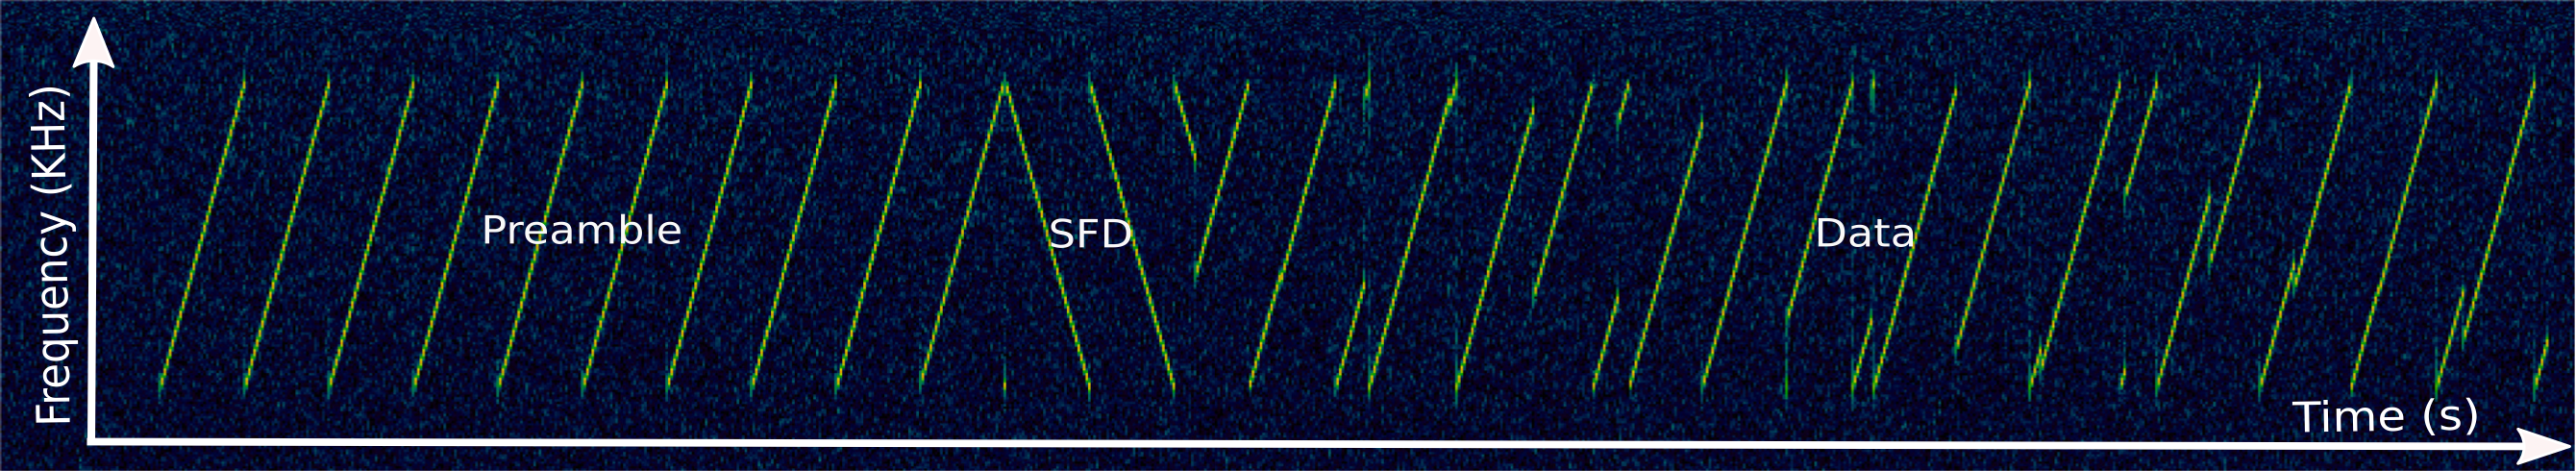
\includegraphics[width=1\textwidth]{chirps}
\caption{A visualized lora packet transmission. Source:~\cite{10.1145/3293534}}
\label{fig:chirps}
\end{figure} \\
In \cref{fig:chirps} we can see ten upchirps (preamble) and two downchirps (start frame delimiter) followed by modulated chirps that contain the actual data. 

(Sources for \cref{sec:lora} are~\cite{10.1007/978-3-030-01168-0_11} and~\cite{10.1145/3293534})

\section{Pycom 4 and Micropython}
The hardware component of this project is a device that runs on little energy and is capable of sending and receiving packets using LoRa technology. The devices represent the nodes in the network. The specific type chosen for this project is called 'LoPy 4'. Additionally to being able to communicate over LoRa, it can also receive data over bluetooth and WiFi.~\cite{LoPy} To be able to connect it to a computer, an additional board - the 'Expansion Board v3.0' - is used where the LoPy device can be connected to. Among additional functionality (LED status light, microSD card slot and further additions) this board has a USB port that can be used to power the device and to upload programs to it.~\cite{ExpansionBoard} \\
The code written in this thesis uses the language Micropython which uses for the most part the same syntax as normal Python. It is a smaller version of Python using only a subset of its libraries and is specially optimized for microcontrollers. \cite{Micropython} \\
While in this project LoPy 4 devices were used, any other device that can run Micropython and has LoRa capability - and similar memory size and other specifications - should be able to run the code written for this thesis and be deployed within the same network.
\begin{figure}
\centering
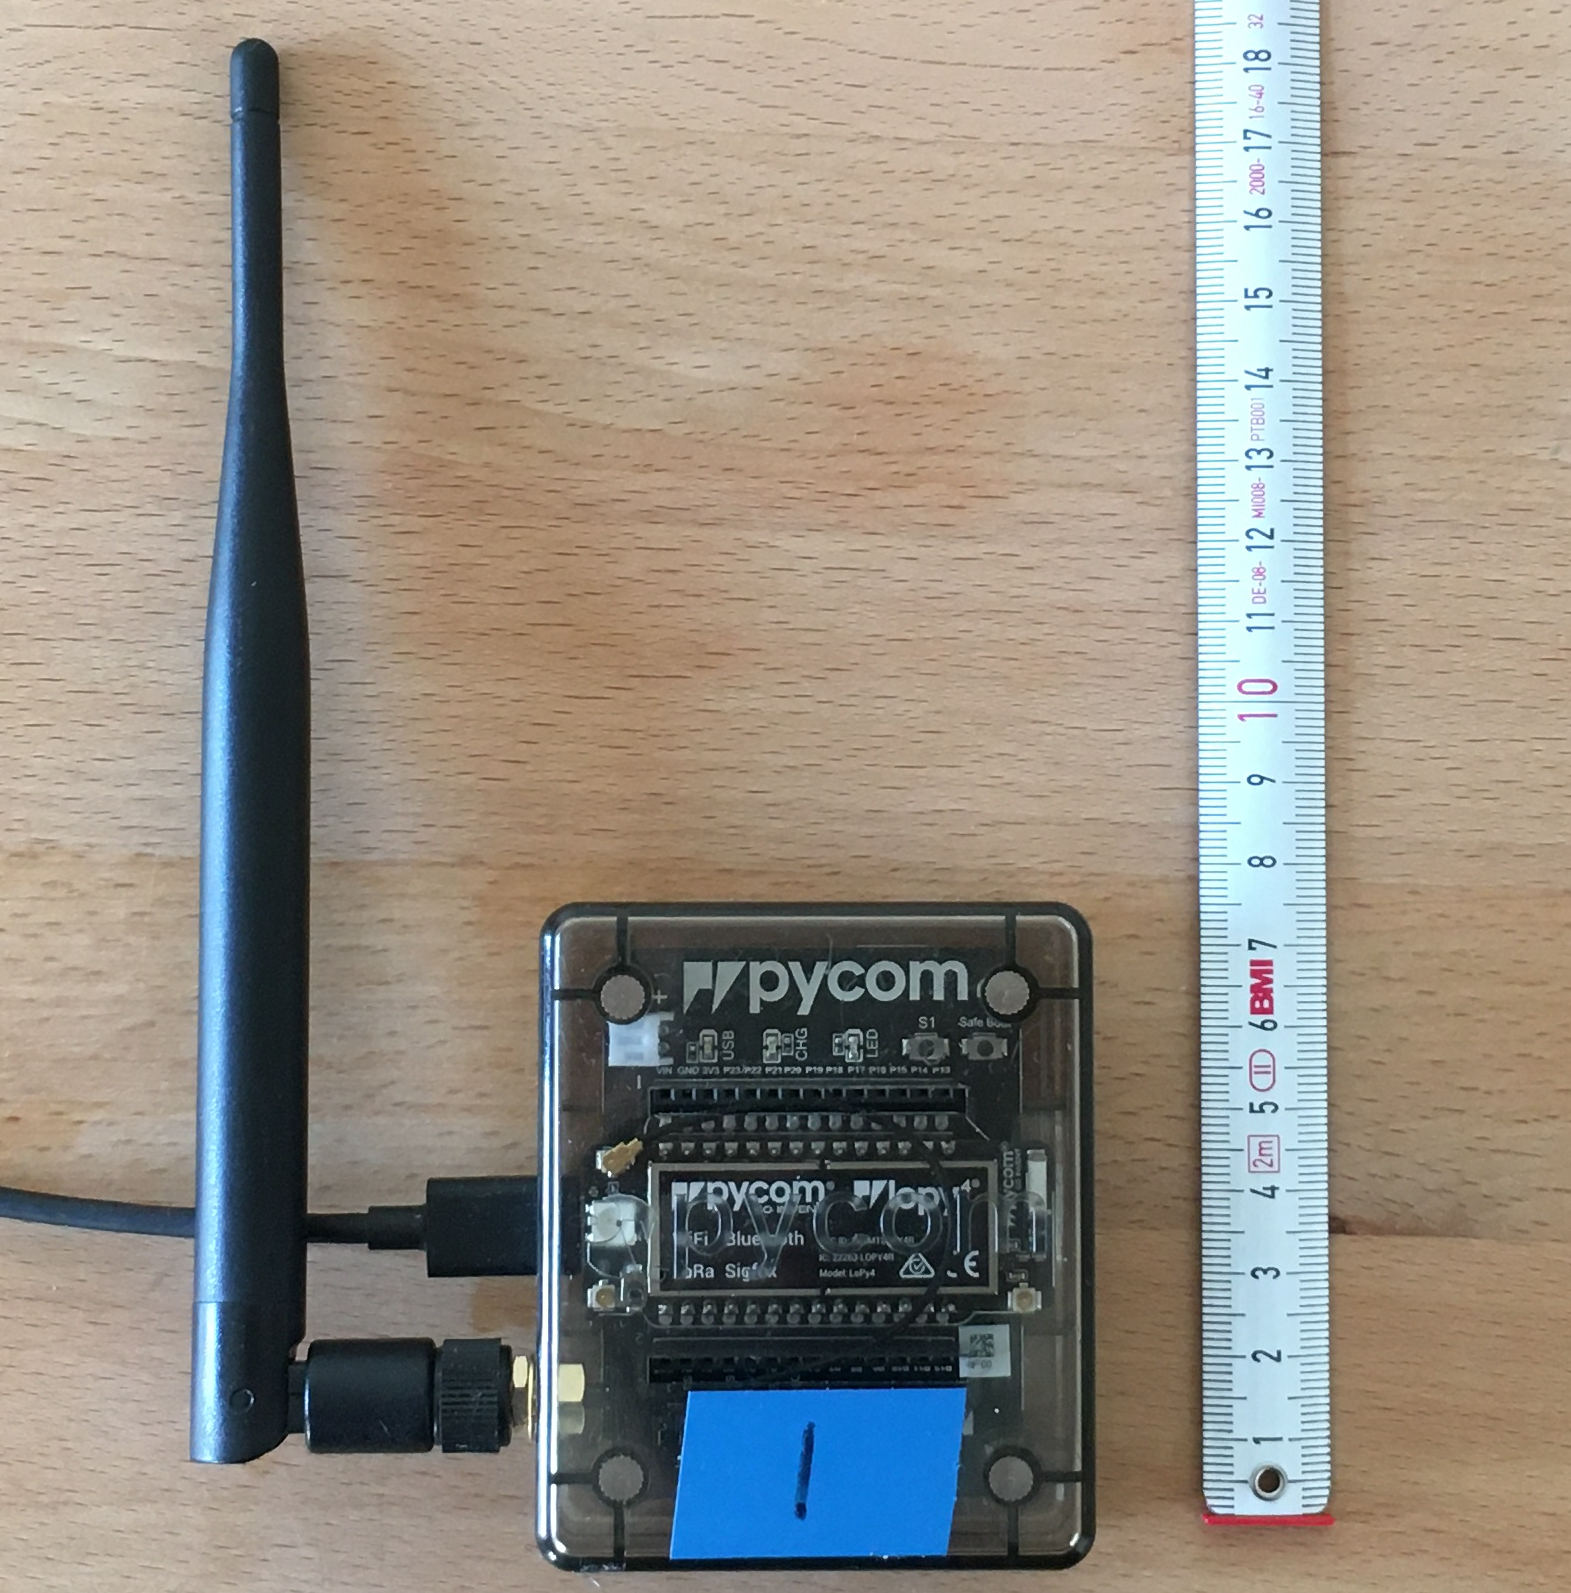
\includegraphics[width=0.45\textwidth]{lopy4}
\caption{A LoPy 4 device used in this project attached to an Expansion Board 3.0 inside a case. On the left side is the LoRa antenna and the cable that can be connected to the computer.}
\label{fig:lopy4}
\end{figure}

\newpage

\section{Overview of TinySSB}
\label{sec:tiny}
\subsection{Pure25519 Signature and Hash Functions}
Two very important concepts in TinySSB that are used at various different points in the system are signature and hash functions. The importance of signatures will be discussed in \cref{sec:signing}. The algorithm that is used in this thesis is the ed25519 elliptic curve.~\cite{9519456} It is used in TinySSB to digitally sign packets on one device and verify the signature on another device. To be able to achieve this, a key-pair has to be created first. The key-pair consists of a public key and a secret key. The algorithm then takes as input any message (in bytes) and the secret key that was created in the first step. The output is a digital signature. If any individual has access to the original message, the signature and the public key, they can verify the signature and confirm that the message was signed with the secret key that belongs to the public key used for verifying. \\
A hashing algorithm is used to convert a byte message with arbitrary length into a fixed size byte value. It is a deterministic algorithm, meaning that for any input, the algorithm will produce the exact same result every time. It is not possible for anyone who knows the hash algorithm to reconstruct the original input message from the hash value. 
In TinySSB the hmac-sha256 hash algorithm is used. It takes any byte value as input and returns a 256 bytes hash value.~\cite{Kelly2007UsingHH}

\subsection{Signing and Verifying Packets}
\label{sec:signing}
TinySSB (Tiny Secure Scuttlebutt) is a protocol that is heavily influenced by SSB (Secure Scuttlebutt). An important concept of both protocols is the use of 'append-only-logs' or 'feeds'. In TinySSB a feed consists of a 128 byte feed header block containing some general information about the feed and any number of 128 bytes log-entries appended after it. Once a log-entry is appended to the feed it cannot be changed or replaced anymore. This is an important property of this protocol and the reason for it is discussed in \cref{sec:anchor}. Every node has one ID feed to be identifiable and an arbitrary amount of child and continuation feeds.
\begin{figure}
\centering
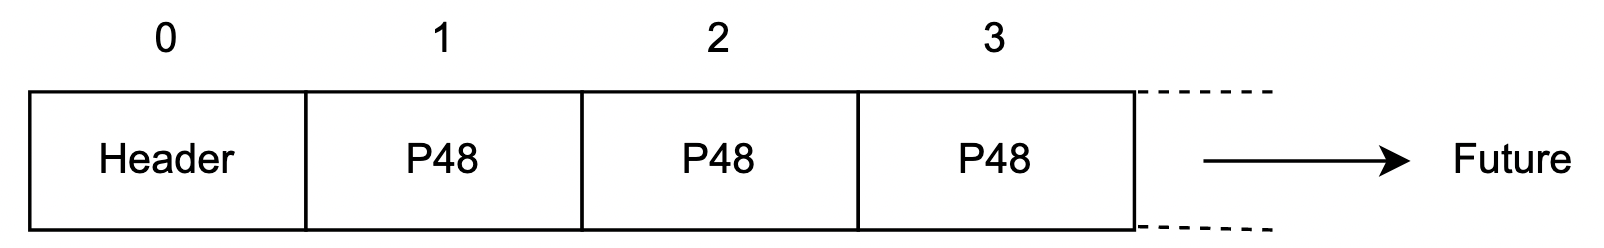
\includegraphics[width=1\textwidth]{feed}
\caption{Feed with the header block and three appended log entries. (P48 describes the standard packet type with 48 bytes payload)}
\label{fig:feed}
\end{figure}

To create a feed, a key-pair has to be calculated first. This is done using ed25519 elliptic curve cryptography.~\cite{9519456} A key-pair consists of a public key - which also serves as the name and identification of the feed (feed ID) - as well as a secret key. These two keys have the following essential property for the TinySSB feed scheme. If a message is cryptographically signed with the secret key, the signature can (only) be verified with the corresponding public key. Every packet that is created and appended to a feed has to be signed by the feed owner with his secret key. This ensures that other nodes in the network - which know the feed ID - are able to verify that a message was indeed signed by the feed owner.

In \cref{fig:packets} we see two packets with the 64 bytes signature appended at the end. The first 8 bytes are not used and reserved for encryption purposes that will be implemented at a later stage. The next 7 bytes are used for demultiplexing. The next byte specifies the type of the packet and the remaining 48 bytes are interpreted differently depending on the packet type. Using the first 64 bytes of the packet, the signature, the public key of the feed and the previous packet, any node in the network can verify the signature and proof that the packet is the correct continuation of the feed. By using parts of the previous packet to create the signature, the trust chain is being continued and for the verifying process the previous packet does not even have to be sent over the network since the receiver already has this packet in its replicated feed.~\cite{tinySSB}\\

\begin{figure}
\centering
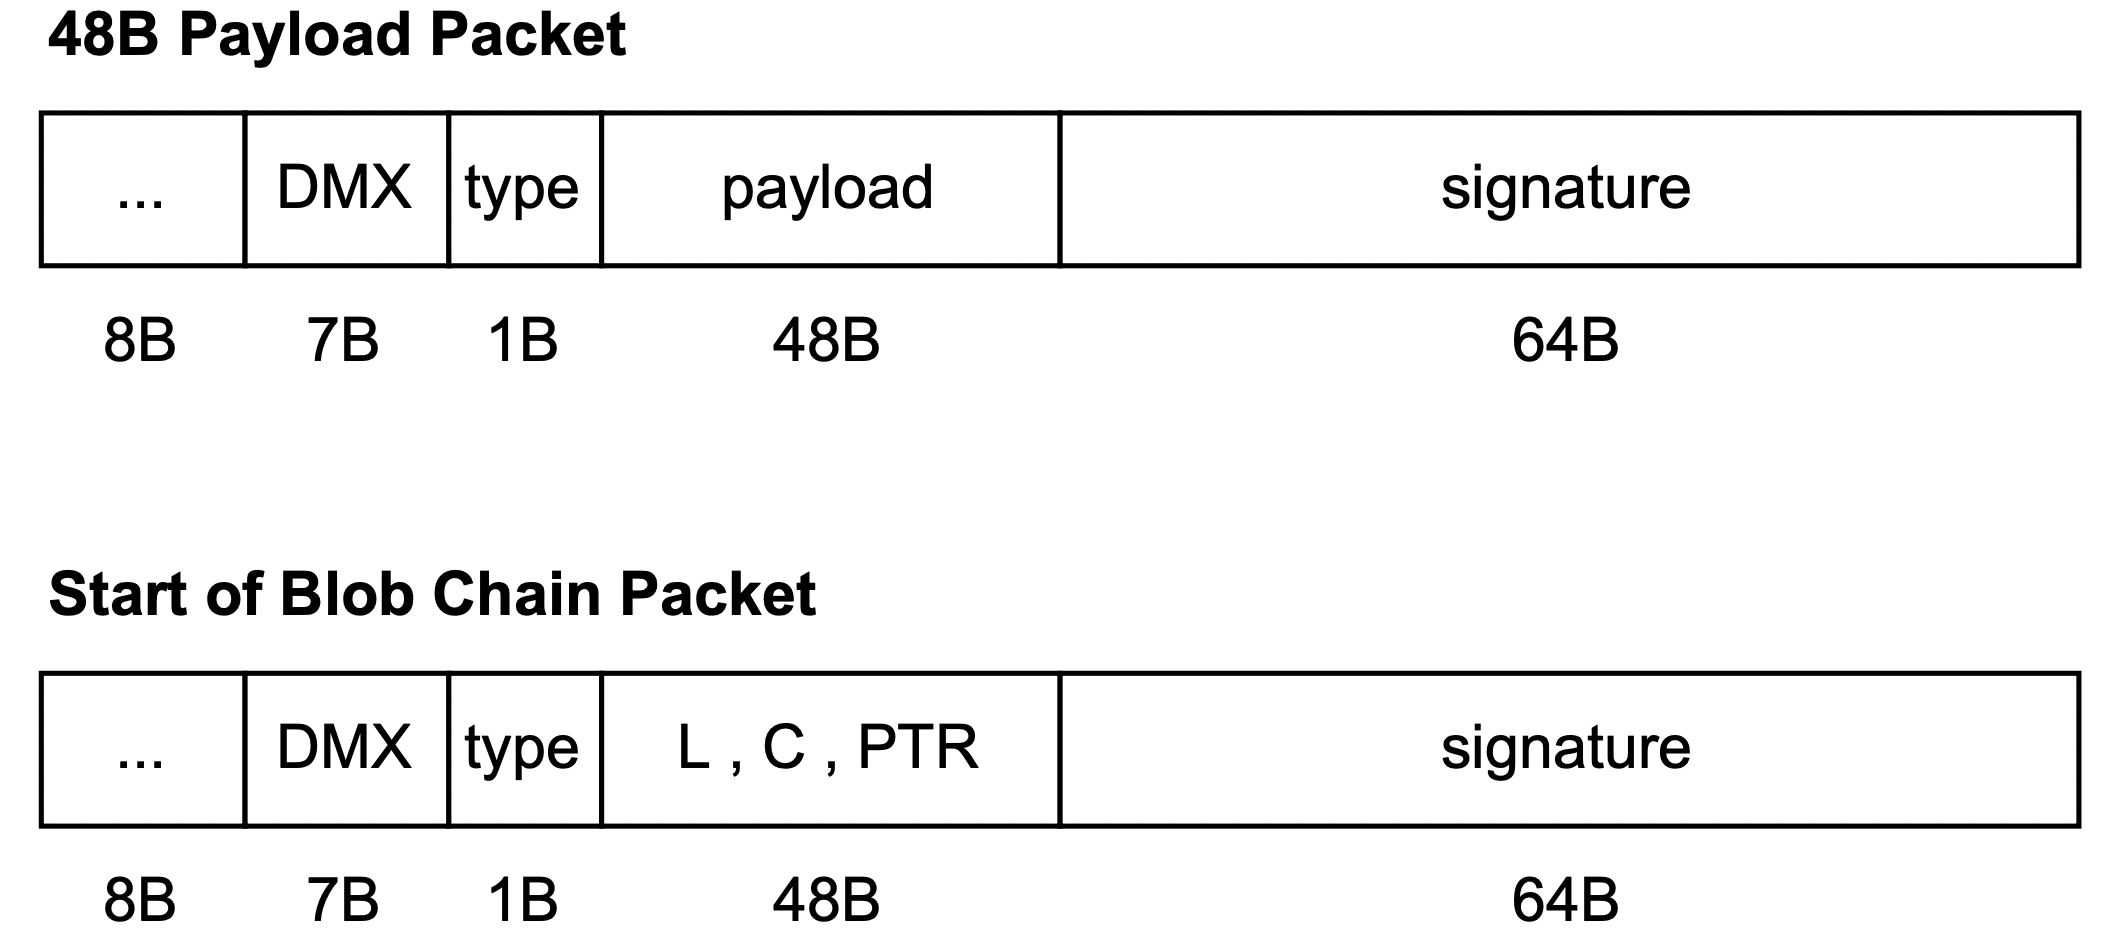
\includegraphics[width=0.9\textwidth]{packets}
\caption{Layout of two different packet types in TinySSB.}
\label{fig:packets}
\end{figure}

\subsection{Sending Data through the Network}
\label{sec:sending}
To propagate data through a TinySSB network, a receiving node has to replicate the feed of the sender. This means that if a feed gets transferred through a series of nodes, in the end every one of those nodes has a copy of the same feed stored on their device (See \cref{fig:replication}). Some feed replicas may be in a different state and have more or less packets appended than others, depending on how fast they can catch up with the feed owner. As explained in \cref{sec:signing}, while replicating the feed, every node has to verify the signature of every packet starting at packet one up until the last packet in the feed. Suppose one node does not verify a malicious packet or intentionally appends a wrong packet to the feed, nodes that will receive those altered packets will not be able to verify them with the feed ID and therefore instead of appending them to the feed drop them immediately.

\begin{figure}
\centering
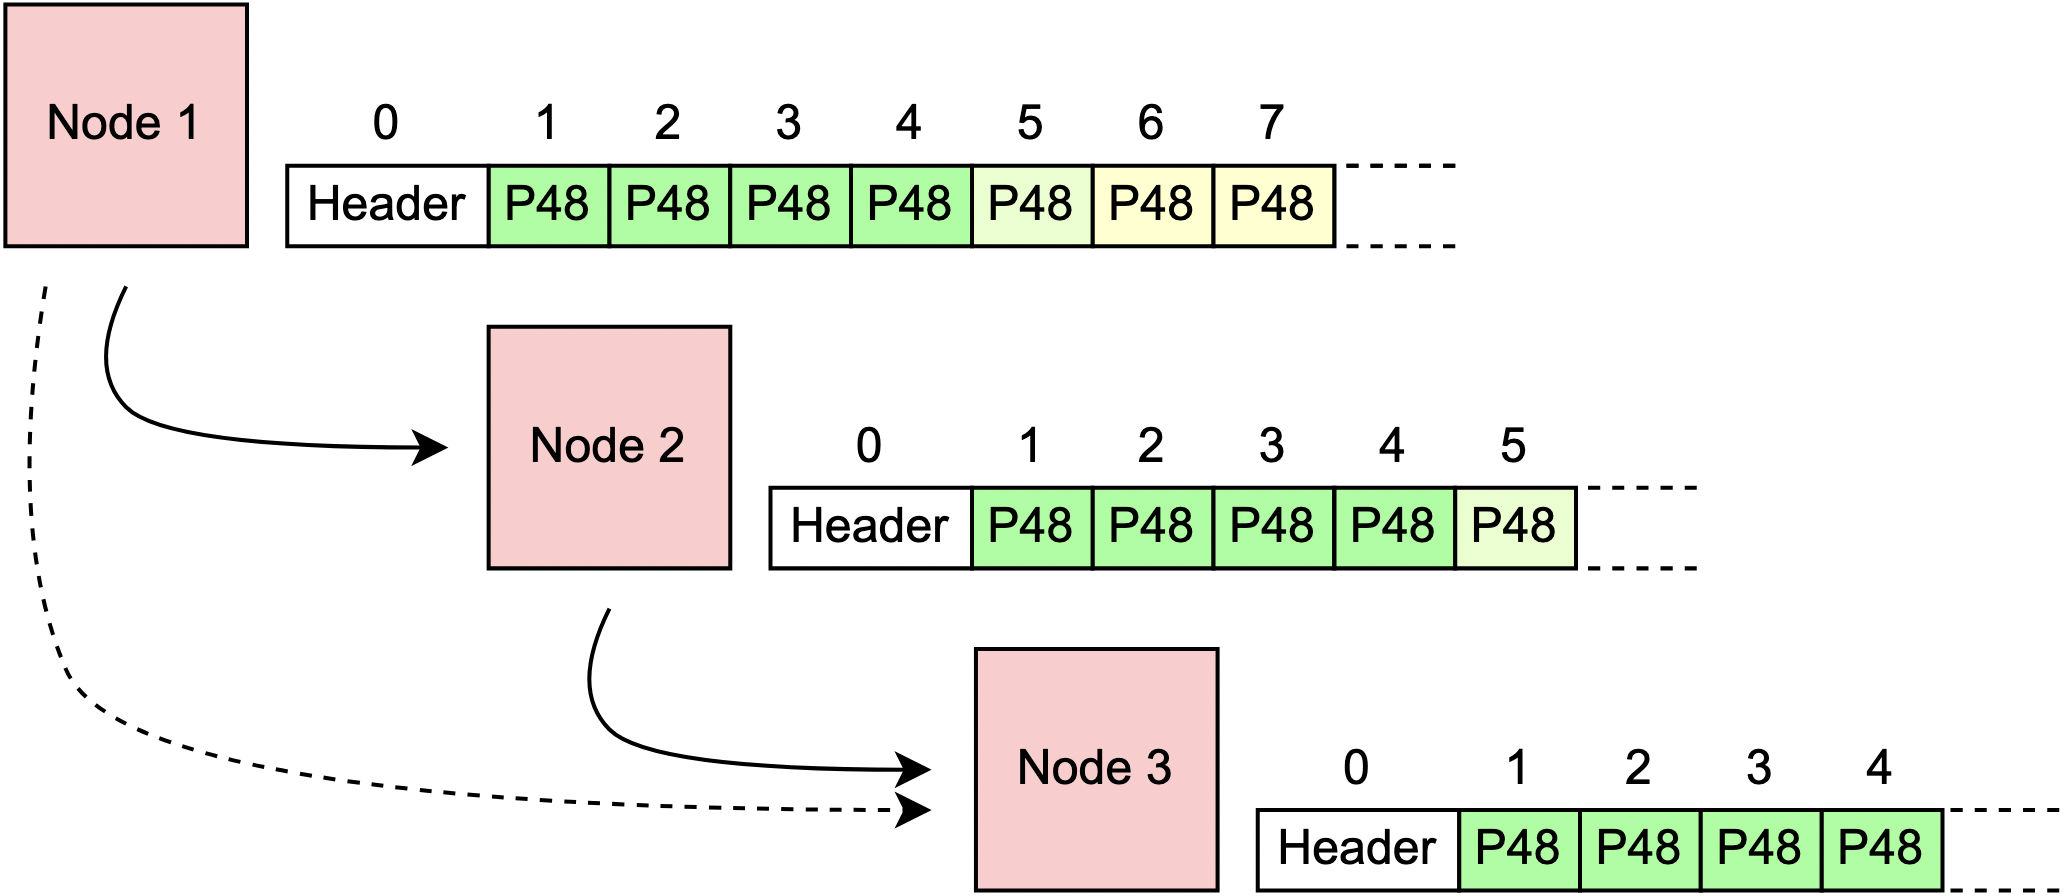
\includegraphics[width=1\textwidth]{replication}
\caption{The same feed forwarded over a series of three nodes. Node 1 is the feed owner and has already appended new packets that are not yet forwarded. Node 2 and 3 create their own replicas and try to catch up with Node 1. If Node 1 and 3 are geographically close enough, packets may even reach Node 3 directly from Node 1.}
\label{fig:replication}
\end{figure}

\subsection{Trust Anchors}
\label{sec:anchor}
In \cref{sec:sending} we explored, how after successful verification nodes can append packets to feeds. Once a node has a replica of another feed, this is a straight forward process. However this does not yet explain how we can start a replication feed. If a node does not know the feed ID of a feed it wants to replicate, it cannot verify and trust the first and therefore also all following packets. To overcome this problem, we have to introduce \textbf{trust anchors}. Before a node can receive any packets from other nodes in the network, it has to be manually\footnote{At least one anchor has to be initialized manually. It would be possible to implement a higher authority / admin feed, that appends further anchors to its own feed and that way propagates anchors through the network.} initialized with trust anchors. A trust anchor refers to the feed ID of an identification feed of a node. If a trust anchor is installed, the node has the ability to verify packets of the corresponding feed and start replicating it. While the first packet of a feed is directly dependent on the trust anchor to verify the signature, all the following packets can be verified with their respective preceding packet. Once it is established that we trust the previous packet, we can also trust the next packet if it has been verified successfully. With this technique a \textbf{trust chain} is built that guarantees authenticity\footnote{No third party can alter the message.} and integrity\footnote{The message can only have been created by the owner of the feed.}.~\cite{tinySSB}

\subsection{Requesting Packets}
An important concept in TinySSB is \textit{how} packets are propagated through the network. Since the whole system builds on append-only-logs, every received packet has to be appended to a log. As a result of this, every node knows which packets it is expecting, namely for every feed stored on the device the packet that follows the currently newest packet. We can make use of this convenient property by creating a list containing a 7 bytes long demultiplexing value\footnote{DMX value is calculated using a hash of the previous log entry, the feed ID, sequence number and a TinySSB specific version prefix.} for every expected packet. With the help of this list, nodes can efficiently handle incoming packets. If the DMX field of an incoming packet is not contained in the DMX list, it can immediately be dropped. If it appears in the list, we can directly try to verify and append it to the corresponding feed. Using this DMX list, it is not necessary to include the feed ID, the sequence number or a backlink to the previous message in the packet. This info is concisely represented in the DMX value and therefore the packet size can be reduced to a minimum. (As opposed to the SSB implementation where this data and some additional information fields are included in every message~\cite{10.1145/3357150.3357396}) \\
Contrary to what \cref{fig:replication} might imply on first glance, network nodes do not arbitrarily send packets and hope that some other node receives them. This would be a very inefficient method. Instead - because nodes know which packets they are expecting - nodes will request the packets with a 'want broadcast'. This broadcast contains the feed ID and the sequence number of the desired packet.\footnote{Instead of the complete feed ID the reduced form sha256(feed ID + b'want')[:7] + seq is sent.} If a node that has the requested packet stored on its device receives such a message, it will send back the specific packet. This scenario is visualized in \cref{fig:request}. If the want request is unsuccessful and no packet is returned, the node has to wait for a given amount of time before trying to request the same packet again. If multiple nodes have the requested packet, they all will return the packet but only the fastest returned answer will be accepted.

\begin{figure}
\centering
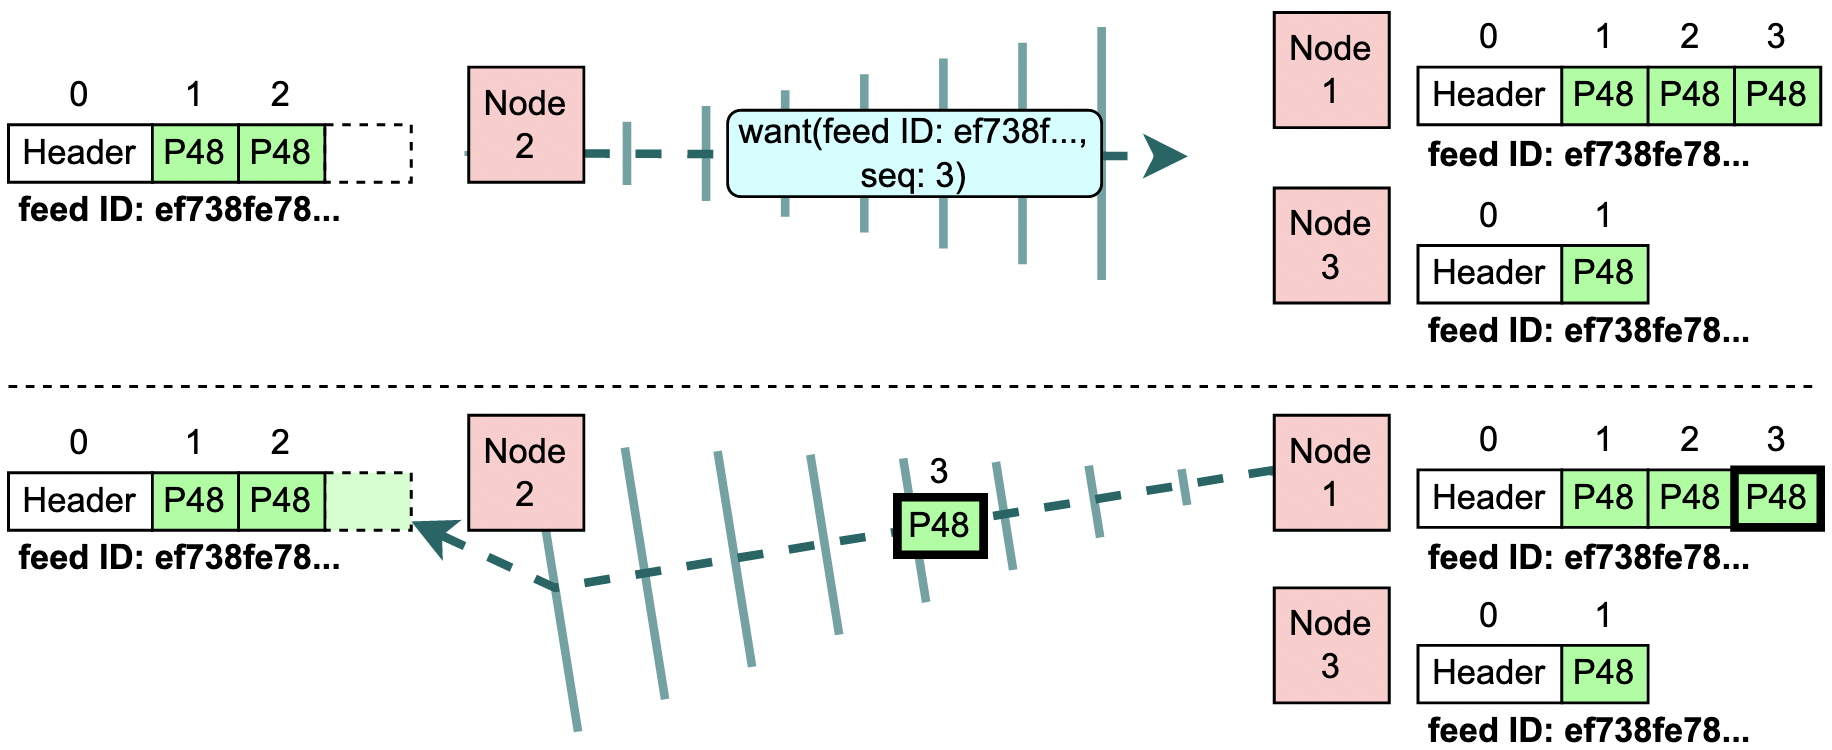
\includegraphics[width=1\textwidth]{request}
\caption{\textit{Top:} Node 2 requests packet with sequence number 3. \textit{Bottom:} Node 1 returns the requested packet. Node 3 does not have the requested packet and therefore does not answer.}
\label{fig:request}
\end{figure}

\subsection{Side Hash Chains}
\label{sec:sidechain}
When using 48 bytes payload packets, the size of data to be transferred is limited to 48 bytes. If it is larger it has to be spilt up into chunks of 48 bytes with the chunks being divided among different consecutive packets. This would lead to a lot of overhead in terms of storage and network use. Therefore a more concise and efficient method - side hash chain - is being used for larger payloads. The data of a hash chain is (for the most part) not stored in a feed. It is stored in a separate location in the file system in 120 bytes sized files. Only the initial packet that points to the start of the chain is appended to the feed as a packet with type chain 20 (See second packet in \cref{fig:packets}). This packet - apart from the DMX, type and signature fields - contains the length of the hash chain, the first part of the payload and a hash pointer to the start of the chain. For chain packets, all fields that are typically used in standard packets can be omitted (except for the first reserved 8 bytes). Of the 120 bytes 100 are used for payload and 20 for the hash pointer to the next chain packet. A hash pointer corresponds to the hash of the next packet in the chain. If the hash value of the incoming chain packet matches the hash pointer of the previous packet, we can guarantee that the packet is the legitimate continuation of the chain. To be able to create such a chain, the sender must start by creating the last chain packet first and and appending its hash value to the second last packet. Then hashing the second last packet to append the resulting value to the third last packet and so forth. This step has to be repeated backwards until the whole payload is split into hash chain packets before the first packet can be sent. A visualization of a side hash chain is seen in \cref{fig:chain}. \\
\begin{figure}
\centering
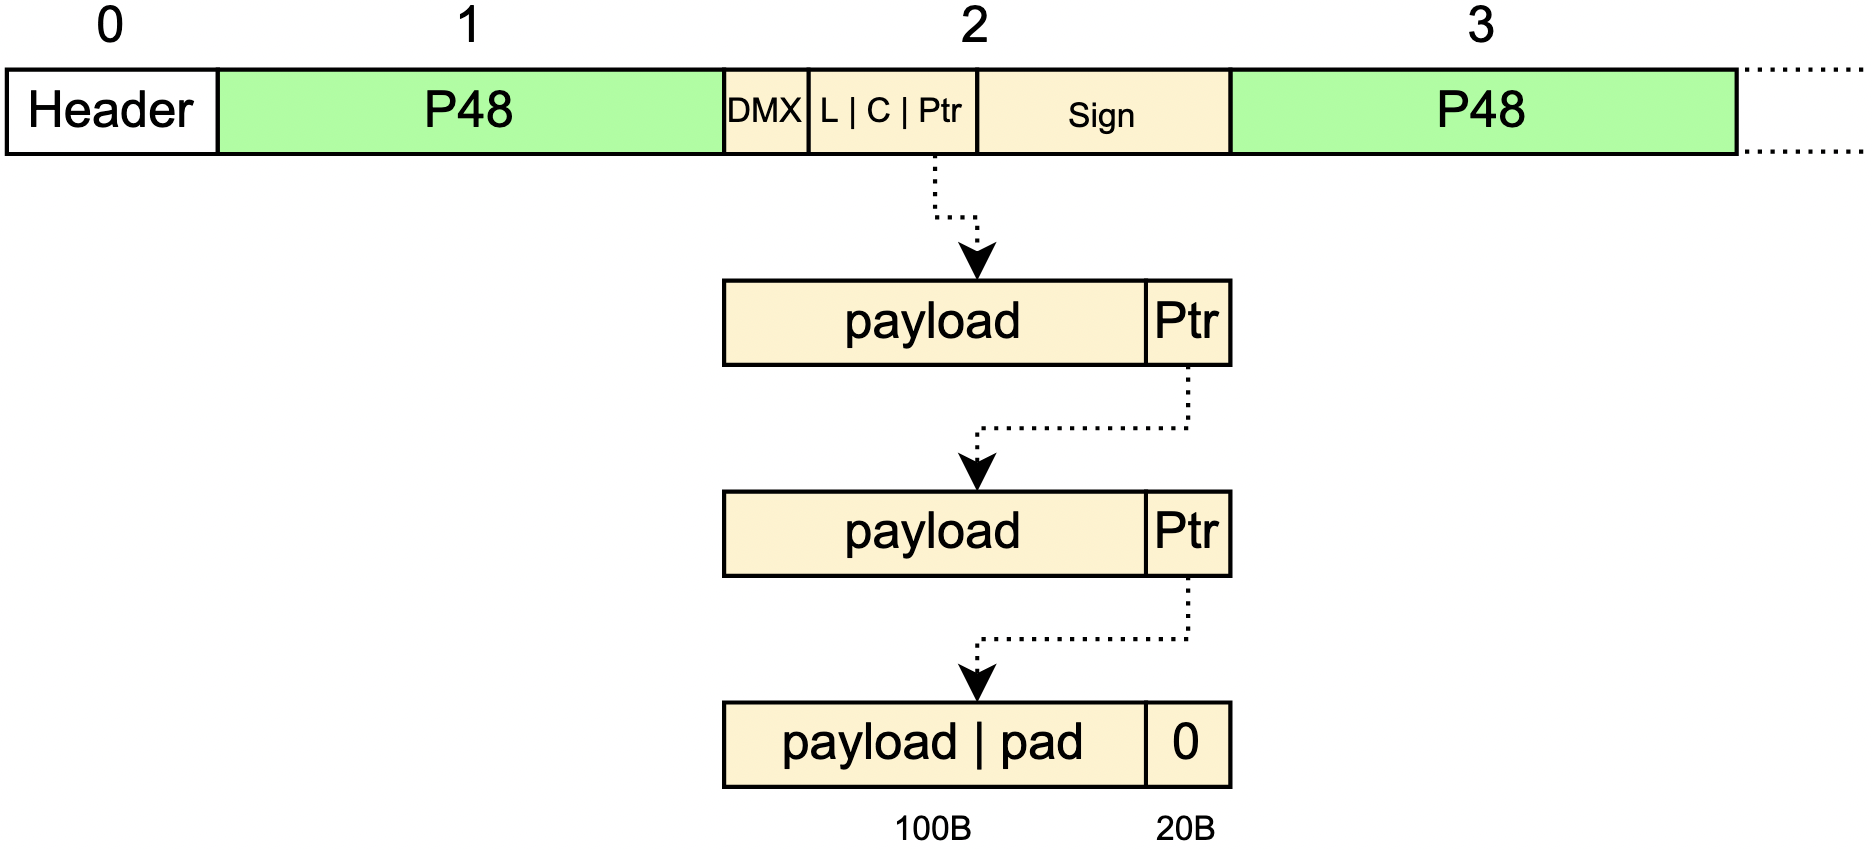
\includegraphics[width=1\textwidth]{chain}
\caption{Feed containing three packets. The second packet is of type chain 20 with a pointer to the next chain packet. In the last chain packet, the pointer is set to zero and a padding is added between the end of the payload and start of the pointer. Matching colors indicate a hash pointer to packet relation.}
\label{fig:chain}
\end{figure}

When a chain 20 packet is at the end of a feed, the whole chain has to be completely loaded before the next packet can be appended. The DMX table must therefore be updated by replacing the old DMX value with the hash pointer to the next chain packet. Thus if an incoming packet's DMX value could not be found in the table, the hash value of the packet has to be compared to the hash pointer values in the DMX table (in a second iteration). To request a chain packet, additionally to the feed id and sequence number, the hash pointer has to be provided at the end of the want request. With those three parameters the correct chain packet can be retrieved given that it is present on the device. \\


\subsection{Creating Child Feeds}
Considering that every node has only its one ID Feed where it appends all data, this one feed could quite rapidly become large, and overloaded with packets of all sorts. To tackle this problem we add more functionality to the append-only-log concept. We add two packet types that are used to create new feeds from within an existing feed. The first packet type declares a new child feed and the second packet type is used in the newly created feed to affirm it is a child feed.

\begin{figure}
\centering
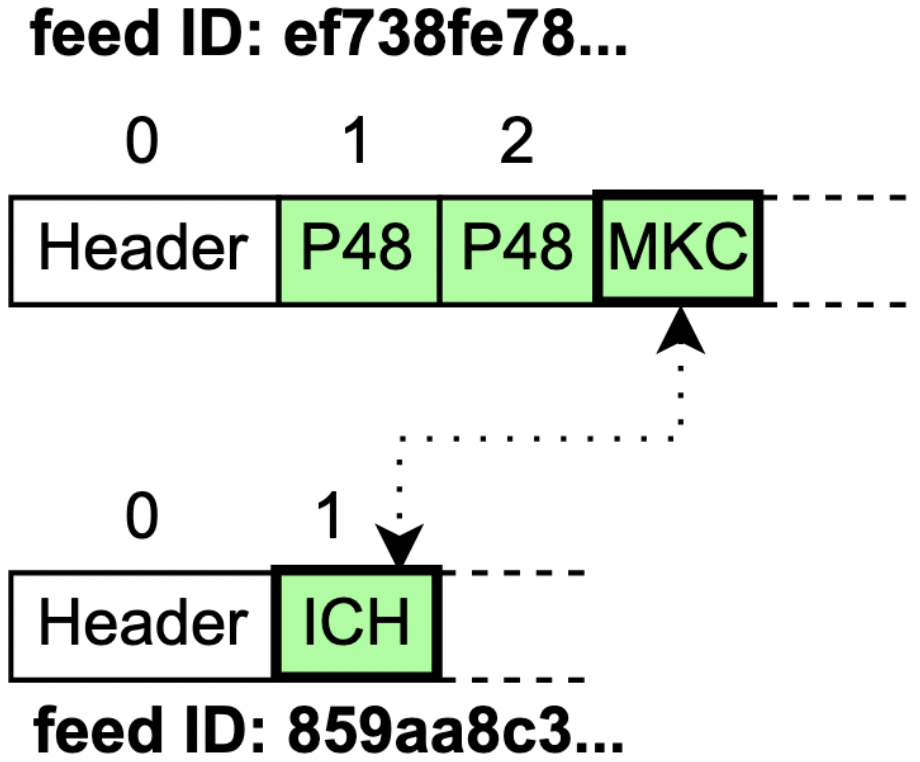
\includegraphics[width=0.4\textwidth]{mk_child}
\caption{The packet MKC declares a new child feed and points to the address 859aa... The packet ICH in the new feed indicates that it is a child feed and has an upward pointer to its parent feed.}
\label{fig:mk_child}
\end{figure}

The advantage of having multiple feeds is not only to separate packets for different applications into different feeds, now the device is also able to request packets for both feeds individually. Depending on the importance of the feeds we can now optimize the request by prioritizing certain feeds over others by sending more want requests for higher priority feeds. Creating a child feed increments the number of entries in the DMX table which has to be carefully managed to not overload the network with want requests. \\
The process of creating a new child feed is similar to creating the ID feed. First a new key-pair has to be created where the public key is used as the feed name and the secret key to sign packets. The node however now has to keep track of the new secret key as well. All key pairs that belong to the node's child feeds are stored in a config file and loaded into memory on start up. If the MKC (make child) packet reaches a node that replicates the feed, it will automatically create and replicate the child feed as well.

\subsection{Creating Continuation Feeds}
A feature with similar functionality is the creation of continuation feeds. The main idea behind this feature is to prevent feeds from becoming too long. There may exist feeds that get appended a lot of data and therefore grow at a rapid pace. When the feed gets bigger than a manageable size it becomes infeasible to propagate the whole feed through the network and store multiple copies of it on every device. For this use-case a packet type that declares a new feed as a continuation and a type that points to the previous feed are introduced.

\begin{figure}
\centering
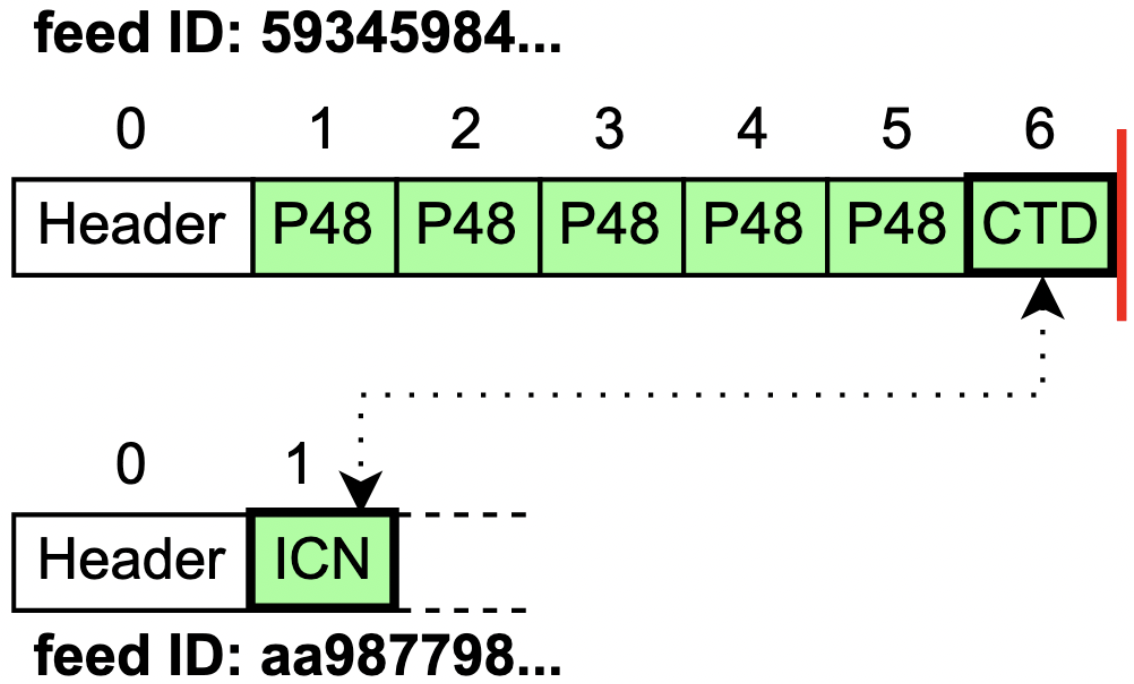
\includegraphics[width=0.5\textwidth]{mk_contd}
\caption{The packet CTD declares a new continuation feed and points to the address aa987... The packet ICN in the new feed indicates that it is a continuation feed and has a backward pointer to its previous feed. The red line indicates that no further packets can be appended.}
\label{fig:mk_contd}
\end{figure}

After a continuation packet is appended to a feed, log entries can no longer be appended, thus new packets for said feed do not need to be requested anymore. However the node still has to respond to incoming want request for the feed to be able to further propagate it through the network. The trust chain in this case is continued through the continuation packets. Using just continuation feeds as in \cref{fig:mk_contd} therefore does not free up storage space or come with any advantage, as still every node needs to build up the complete trust chain (now using two shorter separate instead of one longer feed). How continuation feeds can be useful will be discussed in \cref{sec:session}. As with child feeds, continuation feeds also have their own key-pairs that are stored in the same config file. If the address to the continuation feed is set to zero, this will be interpreted as ending the feed without continuation (No new feed will be created).





%When a group of devices (network nodes) implement the TinySSB protocol, they can together form an independent network. All data that is sent and received over this network is stored in 'feeds'. Every network node needs to have its own key-pair consisting of a public and a secret key. Those two keys are mathematically related to each other and are later used to sign and verify messages. The secret key must be kept secret and not be distributed to other parties. The public key however can be propagated to other nodes. 

%In both protocols the creator of a message must be able to digitally sign messages while the receiver must be able to verify signatures. 






%\section{Tables}
%Some tables can also be used as shown in \cref{tab:table}\footnote{Table captions are normally above the table.}. Remember that tables might be positioned elsewhere in the document. You can force positioning by putting a \texttt{ht!} in the definition.

%\begin{table}[ht!]
%\centering
%\caption{Frequency of Paper Citations. By the way: Make sure to put the label always after the caption, otherwise \LaTeX{} might reference wrongly!}
%\begin{tabular}{lcl} \toprule
%Title&$f$&Comments\\ \midrule
%The chemical basis of morphogenesis & 7327 & \\ 
%On computable numbers, with an application to the ... & 6347 & Turing Machine\\
%Computing machinery and intelligence & 6130 & \\ \bottomrule
%\end{tabular}
%\label{tab:table}
%\end{table}




%\section{Figures}
%Figures are nice to show concepts visually. For organising well your thesis, put all figures in the Figures folder. Figure~\ref{fig:machine} shows how to insert an image into your document. \Cref{fig:tm} references a figure with multiple sub-figures, whereas the sub-figures are referenced by \cref{fig:tm:tm1}, etc. \todoMissing{Description of figure.}

%\begin{figure}
%\centering
%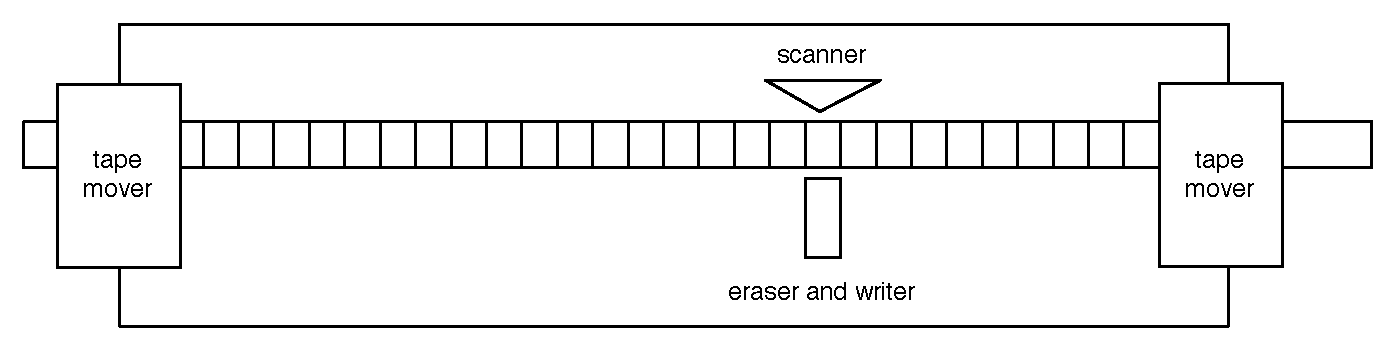
\includegraphics[width=0.9\textwidth]{turingmachine}
%\caption{A Turing machine.}
%\label{fig:machine}
%\end{figure}


%\begin{figure}
%\centering
%\subbottom[Turing Machine 1\label{fig:tm:tm1}]{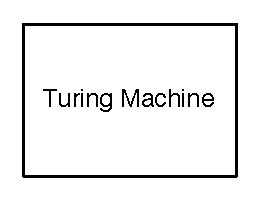
\includegraphics[width=0.2\textwidth]{block}}
%\subbottom[Turing Machine 2\label{fig:tm:tm2}]{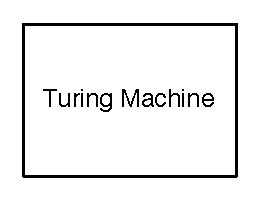
\includegraphics[width=0.2\textwidth]{block}}
%\subbottom[Turing Machine 3\label{fig:tm:tm3}]{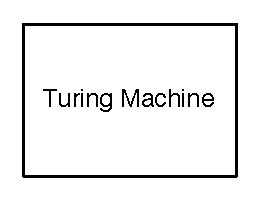
\includegraphics[width=0.2\textwidth]{block}}
%\subbottom[Turing Machine 4\label{fig:tm:tm4}]{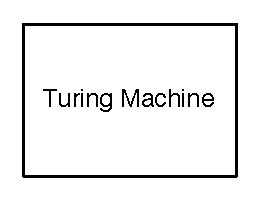
\includegraphics[width=0.2\textwidth]{block}}
%\caption{Plots of four Turing machines}
%\label{fig:tm}
%\end{figure}




%\section{Packages}
%These packages might be helpful for writing your thesis:

%\begin{description}
	%\item[\texttt{caption}] to adjust the look of your captions
	%\item[\texttt{glossaries}] for creating glossaries (also list of symbols)
	%\item[\texttt{makeidx}] for indexes and the back of your document
	%\item[\texttt{algorithm, algorithmicx, algpseudocode}] for adding algorithms to your document
%\end{description}
% !TEX root = ../Thesis.tex
\chapter{Feed Trees}

While feeds are a very powerful concept, there are still some limitations to them. Once a packet is appended it cannot be changed or replaced anymore (this would violate the append-only concept, see \cref{sec:signing}). It is not possible to start replicating the feed at any arbitrary packet position, it has to be built up starting with the header and appending packet after packet until the relevant position is reached (chain of trust, see \cref{sec:anchor}). Since a single feed alone cannot implement those features, we need a different solution. In this section we will explore how we can simulate the desired functionalities using the concepts discussed in \cref{sec:tiny} and some small additions to the TinySSB protocol. By using feeds, child feeds and continuation feeds as building blocks, larger structures can be constructed that are called 'feed trees'. The goal is that the user can interact with those trees on an abstract level as if it were feeds with added functionalities, while hiding the underlying technical complexity.

\section{Fork Tree}
\subsection{Feed Limitations}
If a user realizes that an already appended packets in a feed has an outdated or faulty payload, (s)he cannot revert the append process. A quick fix is to append a new packet to the feed, that informs the nodes to disregard or reinterpret said packet while evaluating it. However the packet stored on the device itself cannot be altered and the fix can only be applied, once the packet containing it has arrived at the node. It also means that newly deployed nodes that replicate the feed have to first receive and append the faulty packet before receiving the fix (chain of trust) even though the feed owner could have created the packet with the fix long before. If not only one but a series of packets have flaws, additionally to the problems stated before, storage would be needed for a lot of undesirable packets. In an autonomous environment especially with only low storage availability, this will be a problem. A different fix is to completely abandon the feed and resend every packet with the updated fixes. While solving the storage problem, it has the disadvantage of taking a lot of time and using the network for sending packets again that were already sent before. Both methods are not desirable and therefore a more efficient solution is presented in this section. 

\subsection{Initialization}
To address the problem of reverting to an earlier position in a feed, the feed structure named 'fork tree' is introduced. A new packet type 'make-fork-tree' is added to the other TinySSB packets. It has technically the same functionality as the make-child packet since it also creates a new feed and points to it. However the packet also triggers TinySSB to create a new fork tree construct. To initialize the tree, three operations have to be performed. First the feed that is pointed at by the make-fork-tree packet (also called root feed) is created. Secondly an additional child feed gets created by appending a make-child packet to the root feed. And thirdly a payload 48 packet gets appended to the root feed as a placeholder. It is used to make the scanning of a larger fork trees easier and could in future implementations be used to add additional meta data to the tree. A newly initialized fork tree can be seen in \cref{fig:fork1}.

\begin{figure}
\centering
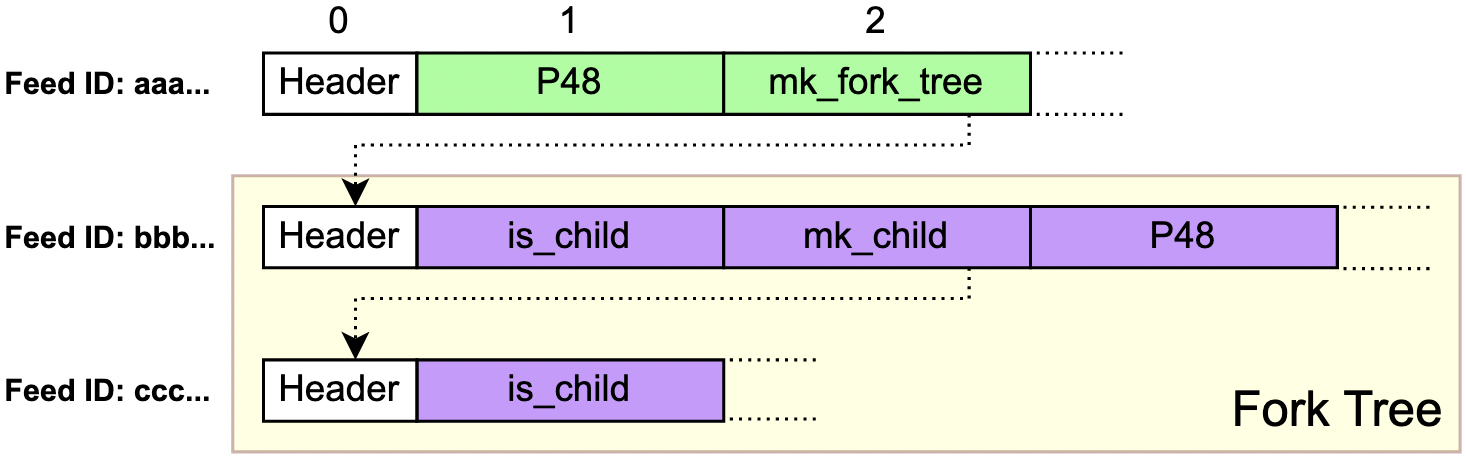
\includegraphics[width=1\textwidth]{fork1}
\caption{Second packet in feed aaa... initializes a new fork tree and points to root feed bbb... . The second packet in feed bbb... creates and points to feed ccc... .}
\label{fig:fork1}
\end{figure}
 
The child feed created from within the root feed is the emergency feed (feed ccc... in \cref{fig:fork1}). If at any point in the future a new fork needs to be created (see \cref{sec:forking}) the appropriate feed will already be present. After initialization the root feed of a fork tree is being used nearly identical to a normal feed. Any packet with either type payload 48 or chain 20 that the user appends to the tree will be automatically appended to the root feed. Other nodes that want to replicate the fork tree could theoretically replicate the initialized tree the same way they would replicate any other feeds and child feeds. However it is only after the structure gets more complex that a new solution must be found (see \cref{sec:dmxfork}).

\subsection{Creating a Fork}
\label{sec:forking}

The idea of creating forks is highly influenced from the ability to fork in version control systems[ADD SOURCE]. Creating a fork in a fork tree means to nominate any packet in the packet chain\footnote{A packet chain can be distributed over multiple feeds. It consists of only the payload packets that were appended by the user. A fork can revert a series of packets and therefore remove them from the chain.} to be the new front packet of the tree. All packets that were appended later are disregarded and can even be discarded. Any further packet that gets appended to the tree continues directly after the newly nominated front packet. To simulate this direct continuation without violating the append-only concept, the emergency feed gets activated and packets are appended there. \\
To successfully start the new fork two operations have to be performed. As the first step, a new emergency feed gets created by adding a make child packet to the old emergency feed. The old emergency feed is now used as the main feed to append packets to while no packets can be appended to the previous main feed anymore. Secondly a new 'fork' packet type is introduced and appended to the old emergency feed. This fork packet contains the feed ID of the previous feed in the packet chain and the sequence number of the previous packet in said feed. A visualization of a fork can be seen in \cref{fig:fork2}.

\begin{figure}
\centering
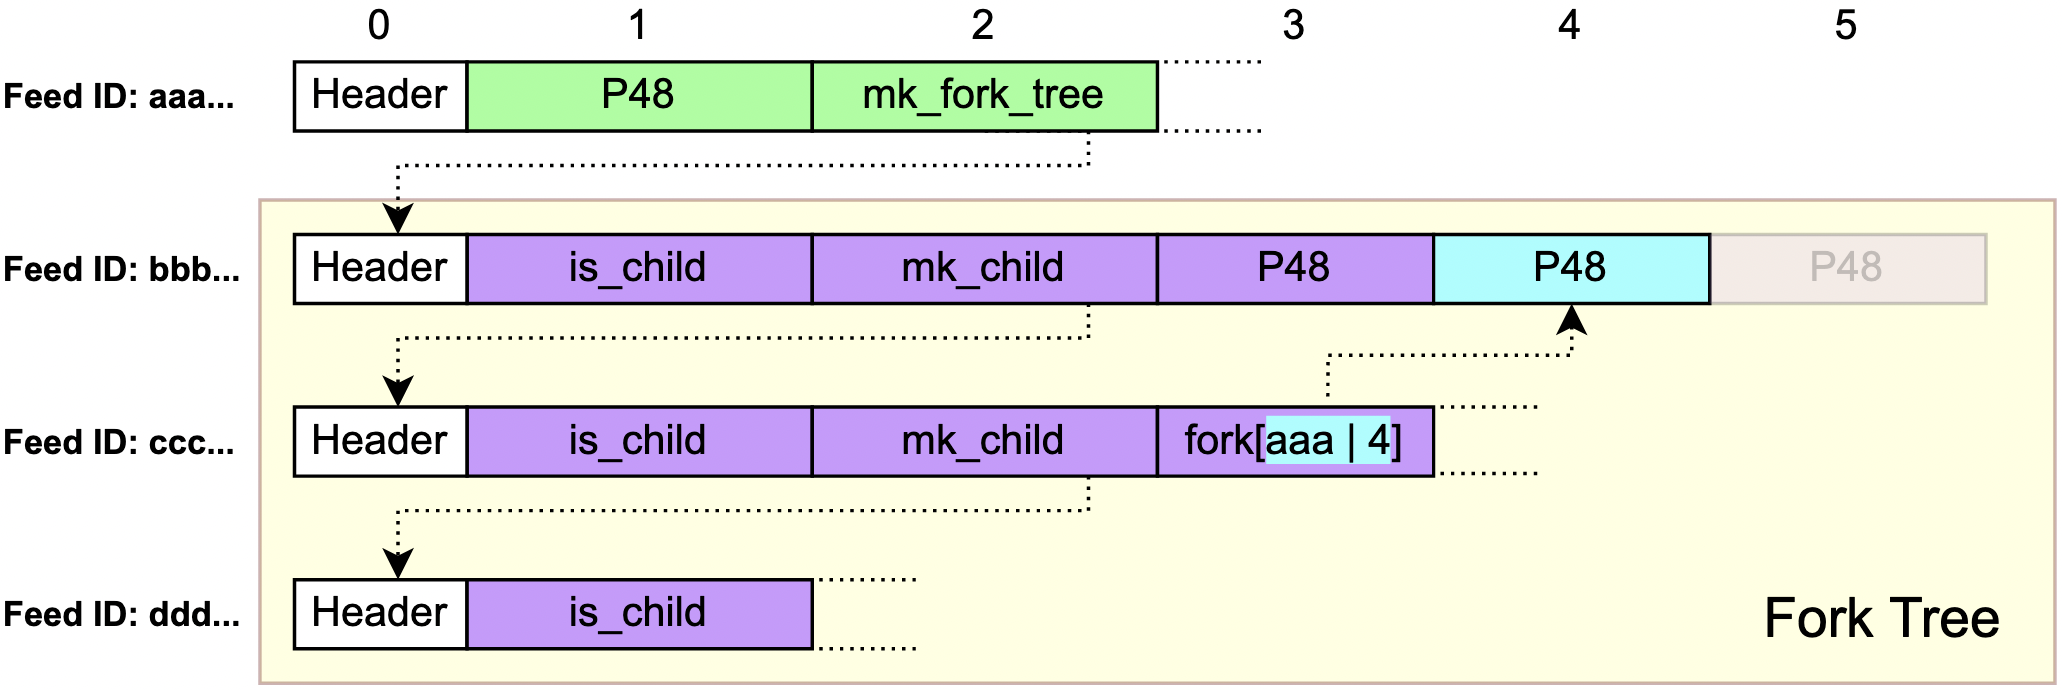
\includegraphics[width=1\textwidth]{fork2}
\caption{Fork Tree with one fork. The fork packet points to the new front packet in feed bbb... seq. nr. 4. Packet with seq. nr. 5 in feed bbb... is disregarded since it was added after the new front. No more packets can be appended to feed bbb... .}
\label{fig:fork2}
\end{figure}

A fork packet does not necessarily have to point to the previous feed. This is demonstrated in \cref{fig:fork3}. The second fork that was created in this example points to a packet before the first fork position. A fork can be created for any packet in the current packet chain except for the one in the front position (this would not revert any packets and only create an unnecessary additional feed).

\begin{figure}
\centering
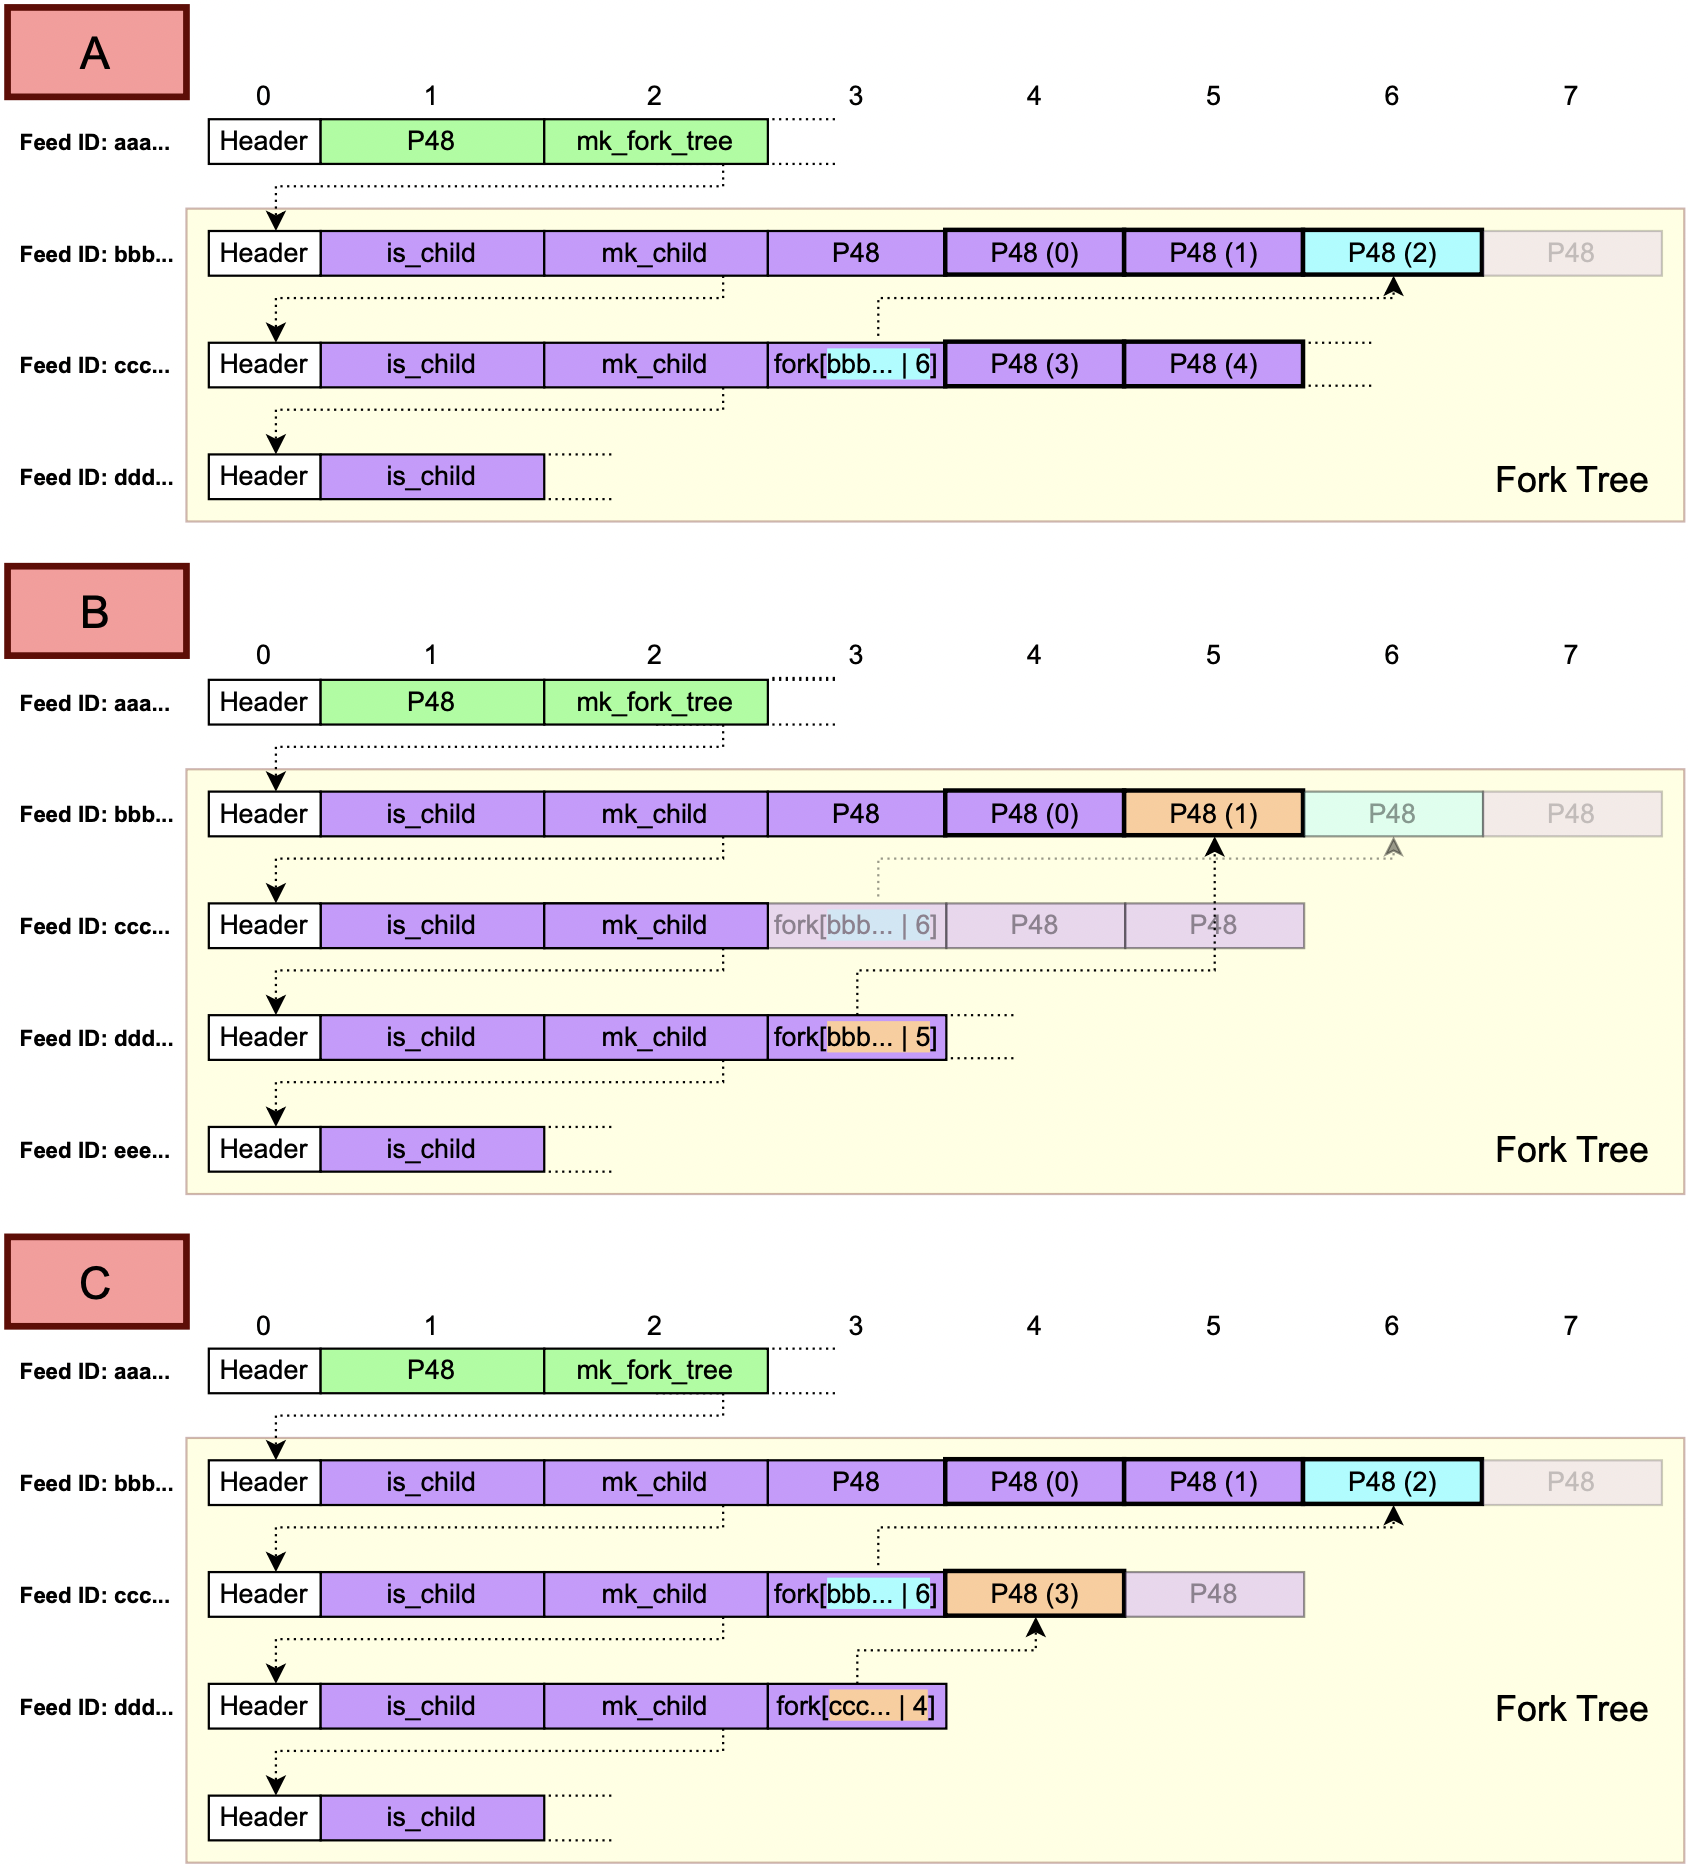
\includegraphics[width=1\textwidth]{fork3}
\caption{Fork Tree with one fork is presented in A. Packets with bold borders belong to the packet chain. The number in parenthesis describes their position in the chain. Transparent packets have been removed from the active tree by the forks. In B the same tree as in A with a new fork appended which points to an older version than the first fork is depicted. By forking a second time the last three packets are being dropped out of the chain and the first fork packet is not needed anymore. In C the tree from A is being forked at a newer position than the first fork.}
\label{fig:fork3}
\end{figure}


\subsection{Producer vs Consumer}
The functionalities discussed in \cref{sec:forking} mainly apply to the producer side\footnote{Node of the feed owner.}. On this side the newest state of the tree is always present, since it is created directly on the node without any transmission delays. However on the consumer side\footnote{Any Node that replicates the tree.} things get a little bit more complicated. The consumer slowly builds up the entire fork tree with packets received over the LoRa network. It is however not guaranteed, that the packets will be received in an optimal order. Situations may occur where a fork packet has already been received, but the packet it points to is not yet present in the tree. Therefore consumer nodes must after appending a packet to the tree always check if the tree is in its current state a valid fork tree. A fork tree is valid if \textbf{(1)} it has at least two feeds, \textbf{(2)} the last feed is set up as an emergency feed (only contains a header and a is-child packet) and \textbf{(3)} when starting at the newest packet and walking backwards along the fork pointers, every pointer points to a packet that exists in the tree. Tree validity does not guarantee that the tree is completely synchronized yet with the original producer tree but it guarantees that a valid readable packet chain can be deducted from its current state.

\subsection{Handling the DMX Values}
\label{sec:dmxfork}
DMX values only have to be inserted to the DMX table for consumer nodes. Producer nodes build the tree themselfs and do not need to request updates from other nodes.
After creating a lot of forks, the number of feeds contained in a fork tree can get large. If nodes would add a DMX value for every feed to the DMX table - and therefore request packets for every feed in the tree - a lot of effort would be used by the node to send want requests for only a single tree. To optimize this, feeds that are not used anymore can be removed from the DMX table. In fact the number of DMX values per fork tree can be reduced significantly. A DMX value for the current main feed and one for the emergency feed are needed at all times to be able to append new packets and to switch to a new fork if needed. If the tree is not valid yet, feeds that have not appended packets until the packet at the position they are forked, need to be added to the DMX table. If in \cite{fig:fork3} C feed bbb... had only appended packets until sequence number 3, the DMX value must stay in the table until the packet with sequence number 6 is appended. As soon as the forked position is appended, the DMX value can be removed for this feed.


\section{Sliding Window Tree}

% !TEX root = ../Thesis.tex
\chapter{Resource Management}
Resource Management is an important part when using autonomous devices which only run on low energy. Storage and energy limitations both need to be considered when running a TinySSB node. Some aspects of resource management were already discussed in \cref{sec:fork} and \cref{sec:session}. By reducing the number of feeds for which nodes request packets, energy consumption can be reduced. By being able to delete older feeds or packets, storage usage can be reduced significantly.
However there are still options left that can further reduce computing power and memory usage.

\section{Resource Manager Loop}
Scheduling the resource allocation is done in the Resource-Manager-Loop. Its main job is to optimally distribute computing power to four tasks. The first one is specific to the node and includes any computation that the node has to do in order to append data to its own feed. This could be recording the temperature or humidity or any other sensory data and appending it to a feed or tree. If the node only serves as a network node to forward data, this task can be neglected. Secondly it has to handle incoming packets and append them to feeds that the node replicates. Thirdly it has to send want requests for feeds it is replicating and lastly it has to send packets if want requests were being received. After one iteration of the loop has been processed - or in harsh low energy conditions already at places within the loop - the device can decide if it goes to sleep for a certain amount of time (while it still is able to receive packets and append them to the in-queue [see \cref{sec:io}]). In the test cases for this project the nodes slept for 3 seconds before starting the next iteration of the loop. However the focus was not set on energy efficiency. In larger networks, the waiting time for individual nodes can probably be longer to not clog the network and reduce energy consumption.

\section{Incoming and Outgoing Packets}
\label{sec:io}
An important part of resource management happens when choosing which outgoing packets to send first and which incoming packets to read first. Some feeds should be considered as more important than others and therefore should be handled first. However it should still be guaranteed that feeds with less importance get allocated some resources as well. To help solve this problem a new priority queue is introduced. One instance of such a queue is created for incoming packets and one for outgoing packets. If a packet reaches a node, it gets appended to the incoming queue. When a packet is ready to be sent out, it is appended to the outgoing queue. A user has to first define a number $n$ of how many different priority classes should exist. Every priority $p_i$ (from $p_0$ to $p_{n - 1}$ gets assigned a certain amount of slots from the total slot count. A slot is not bound to a time or computation limit but represents one packet request from the priority queue. This slot amount is calculated with the following algorithm: \\ 
$slots_p = \lceil (n - p)^{1.5} \rceil$ \\
For $n = 3$ priority classes this would result in 5 slots for $p_0$, 2 slots for $p_1$ and 1 slot for $p_2$ (with a total slot count of 8). This simple algorithm worked well for the use-cases tested (3 and 4 different priority classes) must however be reevaluated if in a later use-case significantly more priority classes are needed. \\
When adding a packet to a queue, the user can give the packet a priority from 0 to $n - 1$ with 0 being the highest and $n-1$ the lowest priority. When requesting packets from a priority queue, packets are returned according to the slots described before. If 8 packets are requested consecutively from the queue, priority 0 is guaranteed to have at least 5 packets returned, priority 1 two packets and priority 3 one packet. However if no packets exist in the queue for a given priority class, the slot gets transferred to the next higher priority class. To further optimize the queue and to avoid redundancy, packets can only be appended if the same packet is not already in the queue. This is a very important feature since one packet request could lead to multiple nodes returning the same packet. By only processing one packet, the computing time and memory usage can be reduced.

\section{Central DMX handling}
To improve DMX handling (packet requesting and matching DMX values of incoming packets with the DMX table), this is handled in a central DMX filter class that is managed by the resource manager. This filter handles DMX values in different category groups. Every new value has to be added to a specific category. The number of categories is not limited and the node creates a new category for each feed tree and one for ID feeds. This is done to be able to easily delete or change all DMX values of a category or tree with a single command. Since for every expected packet there is a corresponding want request, the creation of want packets is also handled in the same class. When sending a want request, the resource manager can directly ask the DMX filter for a want packet and append it to the out-queue. To prevent the node from asking for the same packet multiple times in a short time, the filter only returns the same want packet after a certain time interval has elapsed.
% !TEX root = ../Thesis.tex
\chapter{Conclusion}
In this thesis the goal was to find ways of improving the resource management and thus reduce storage and energy usage as much as possible while still having a system that lets us create a reliable network consisting of autonomous devices. TinySSB was used as a starting point and a resource manager was built on top to orchestrate the activity of TinySSB. While most functionalities of Micropython worked without any problems on the Pycom 4 devices, the pure25519 verifying algorithm - which is an essential part of the project to guarantee integrity and authenticity - initially did not work. After changing a modulo operation we managed to get it working and were able to start testing the network. However verifying one packet still takes a couple of seconds and also quite a bit of computing power. A native implementation in C of this algorithm that can be called with Micropython would probably be a huge improvement in terms of energy consumption. A frequent problem that was occurring were stack overflows. Due to the limited memory capabilities of the Pycom 4 devices a node can quickly overflow its memory. We first tried to verify incoming packets simultaneously in different threads however had to abandon this idea because of said stack overflows. By reducing the use of threads as much as possible, we were able to reduce the stack overflows. Replicating normal feeds or session trees now works without any issues. However for the fork trees stack overflows on the receiver device can still occasionally occur. We could not find a solution for this problem. \\
To reduce the storage size, we first tried to add packet types containing delete or modify commands that a user could manually append to a feed and with it remove or change older feeds. However we quickly realized, that this method would be very complicated and not generic enough to easily be replicable in different situations. The introduction of feed structures that handle storage management automatically was therefore a better suited path to take for our situation. The trees is the current state disregard unused feeds or packets. Deleting a feed only deletes it from memory but not from the device storage. While the construction of feed trees on the producer side was rather simple to implement, complications started once we tried to replicate them in the network. A lot of unexpected situations occurred because the structure on the receiver node is not at all times a complete tree and we do not know which feed will receive the next packet. We had to account for that and find solutions to cope with those problems. The use of a central DMX table where entries are assigned to categories helped a lot in this regard. It let us update the DMX values for a specific tree without affecting any other feeds on the node and thus could reduced errors in the code. \\
While there are still a lot improvements that can be made to the system [ADD REF], in its current state a functioning network can be deployed.

\section{Future Work}
A lot of settings can be tweaked to optimize the packet requesting. In the session tree for example, feeds on a higher layer or the root feed could be given higher priority. If the priority is too high, a lot of unanswered want requests will be sent. If it is too low, it can take a long time until the tree finally adds a new pointer layer. Maybe dynamically changing priorities can be something that could be looked at. For example if a new packet was appended to the root feed, increase the root feed's priority until the request is unsuccessful. Further session trees may be optimized by changing the number of pointer packets per pointer feed or having only a pointer to a session feed every $x$ feeds. This could reduce the number of pointers while still having a sliding window. \\
Obviously the deletion of feeds from storage must be implemented to be able to let a device run over a long period of time. \\
Further testing a system with more nodes over a long period of time could potentially point to some bugs that have to be fixed before a reliable network can be deployed. And finally connecting it to a solar panel and deploying it outdoors will truly demonstrate if the concept of the system works. \\
%\input{./Chapters/Chapter4}
%\input{./Chapters/Chapter5}
%\input{./Chapters/Chapter6}
%\input{./Chapters/Chapter7}
%% ----------------------------------------------------------------
\thesisappendix
\thesisbib
\begin{appendices}
	% !TEX root = ../Thesis.tex
\chapter{Appendix} 
\end{appendices}
%% ----------------------------------------------------------------
\thesisback
\iflanguage{english}
  {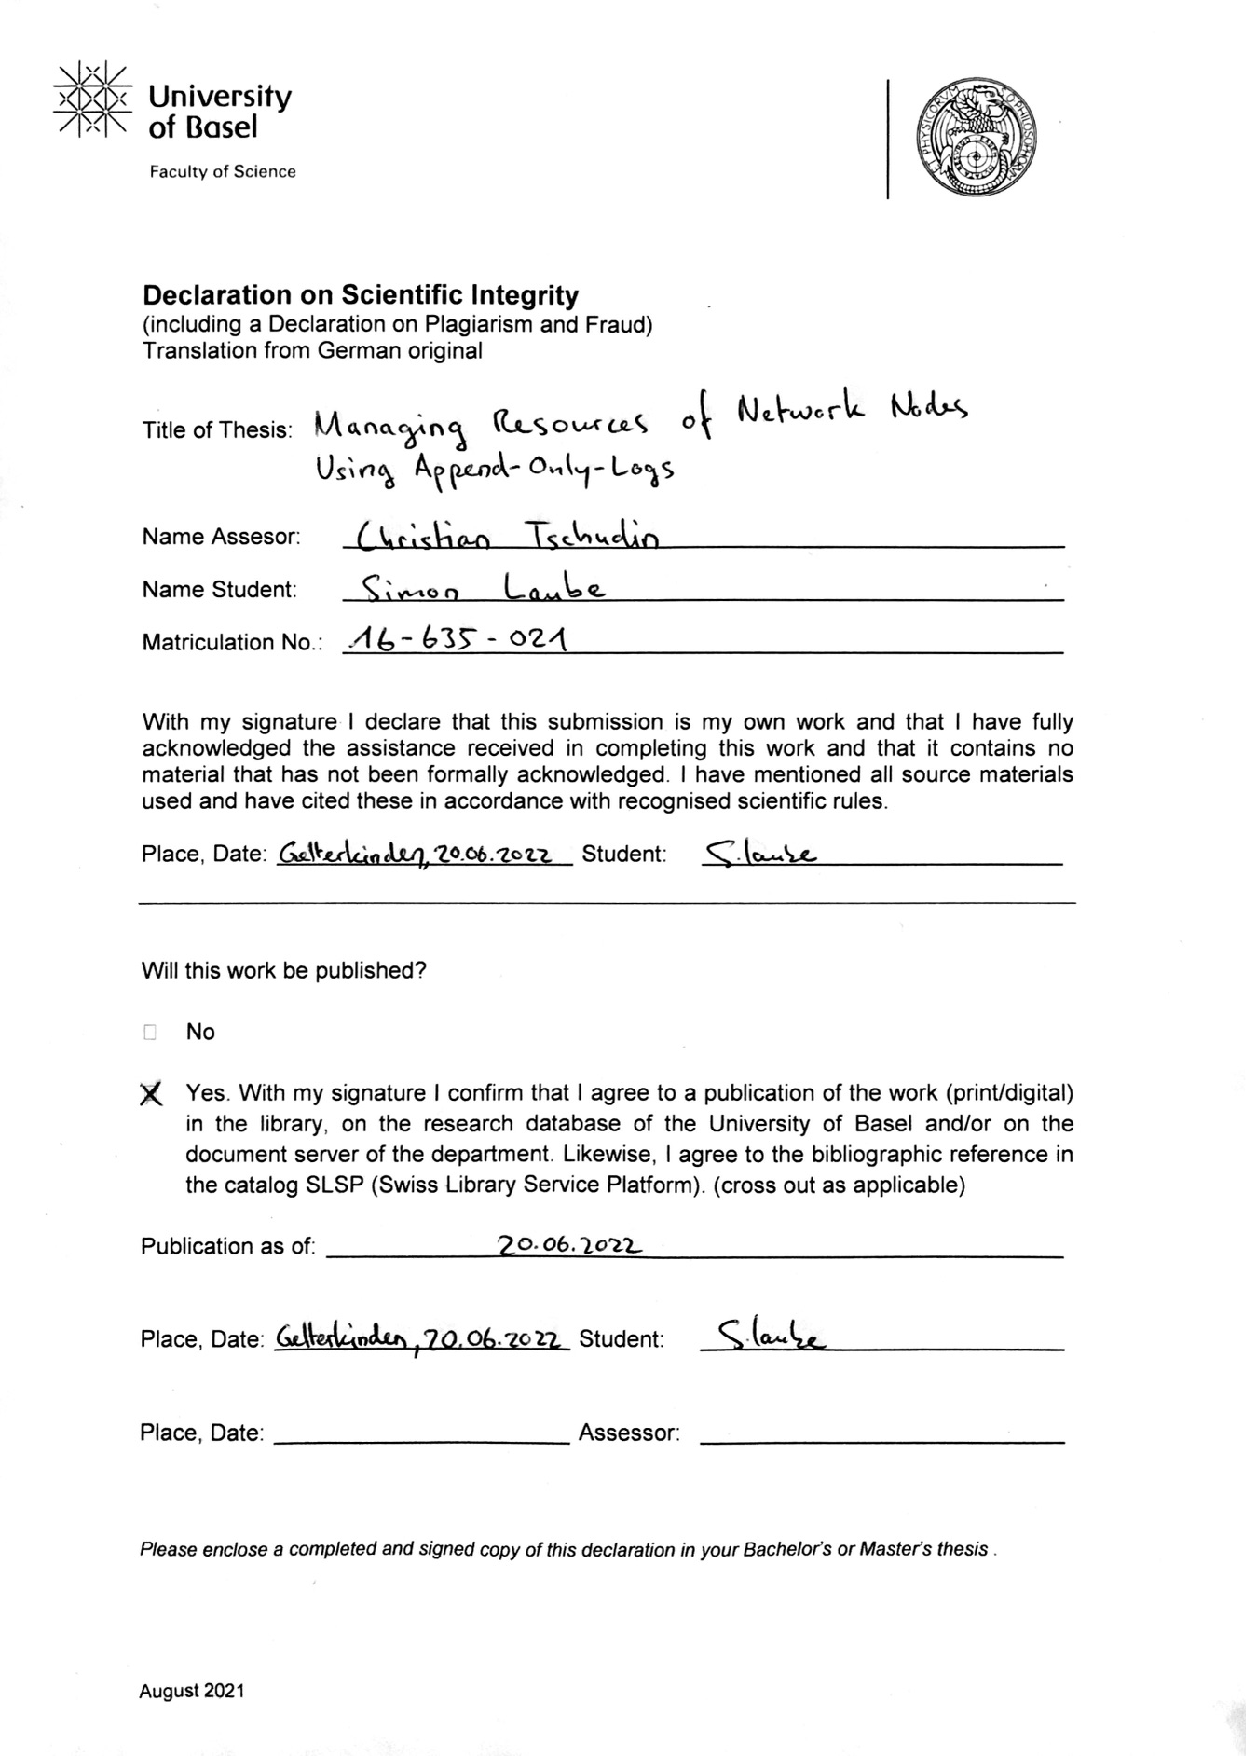
\includepdf{./Back/wissensch_Redlichkeit_E_Aug_21.pdf}}
  {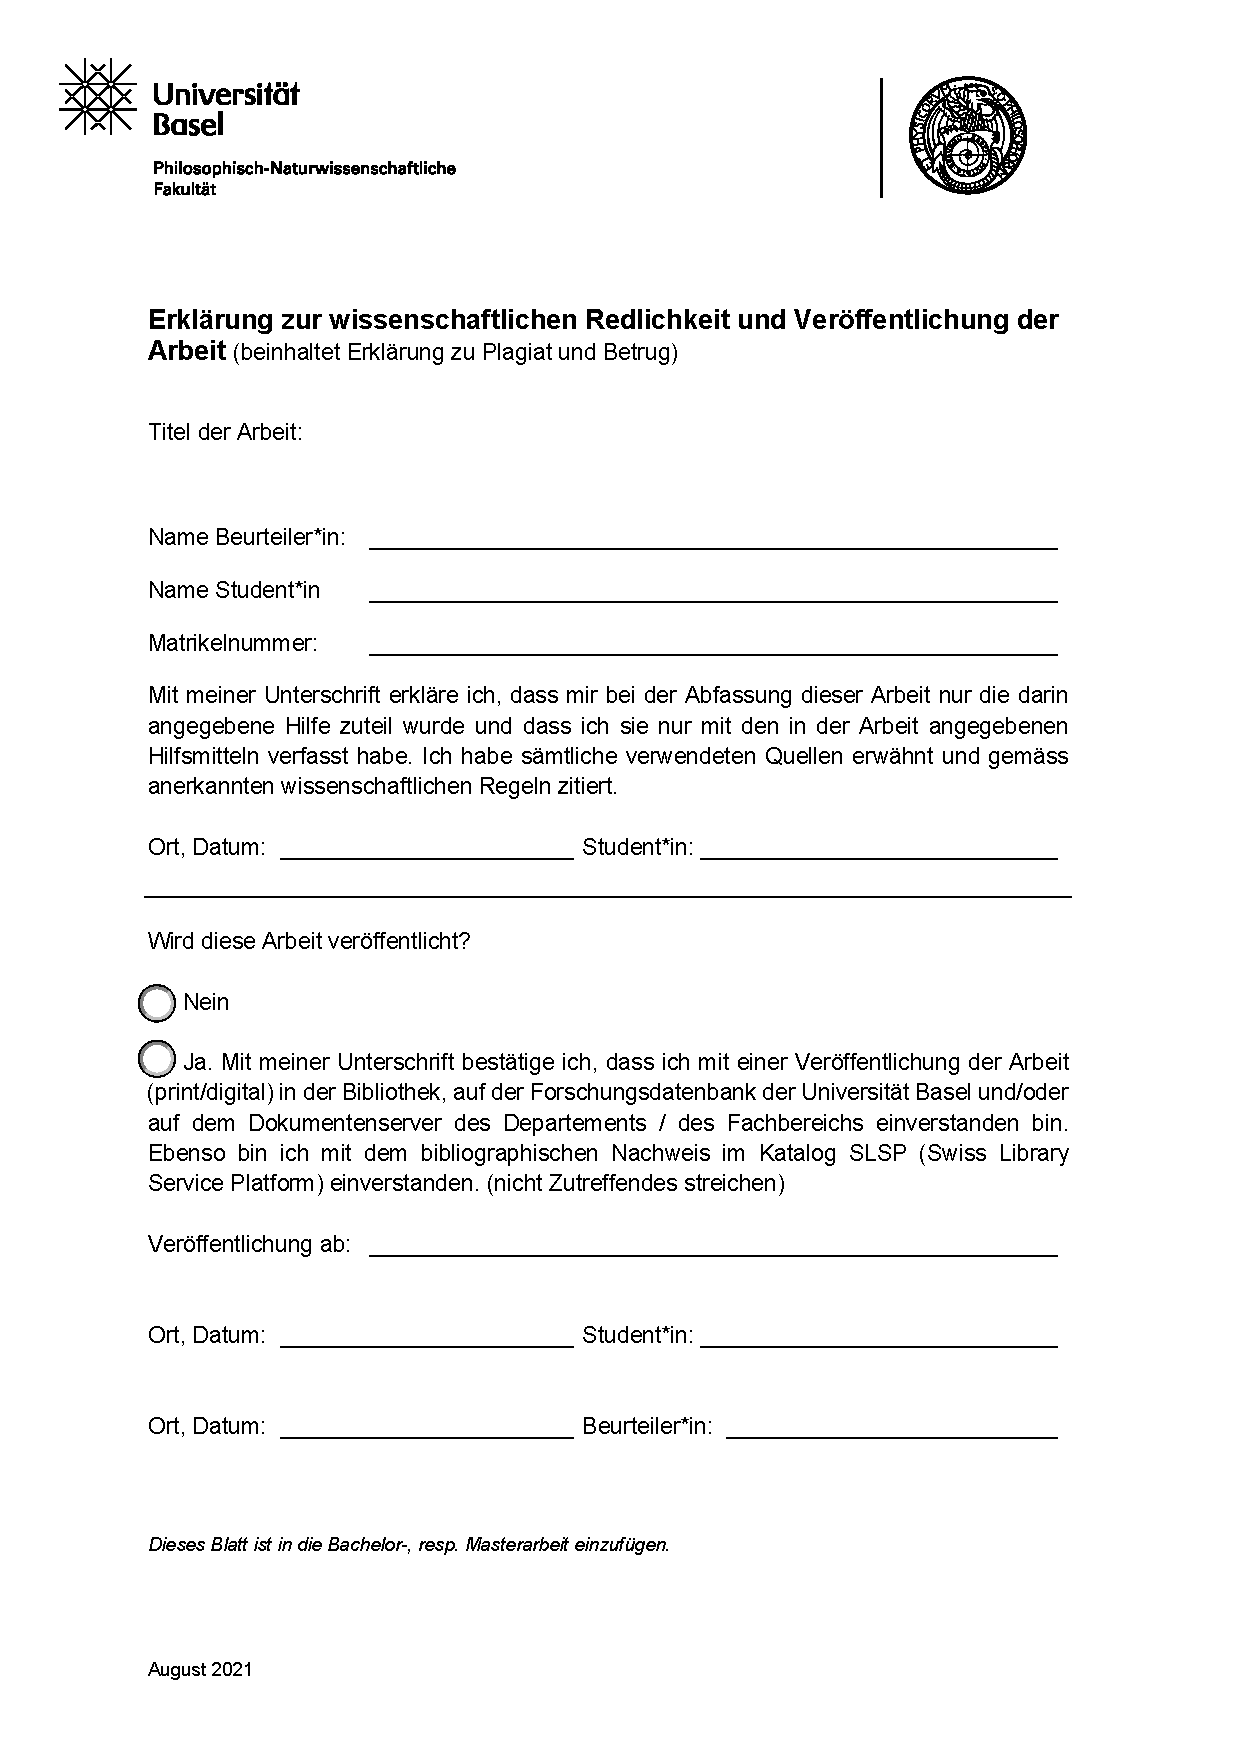
\includepdf{./Back/wissensch_Redlichkeit_D_Aug_21.pdf}}
%% ----------------------------------------------------------------
\end{document}
%% ----------------------------------------------------------------
